\documentclass[a4paper,titlepage]{article}
\usepackage[utf8]{inputenc}
\usepackage[ngerman]{babel}
\usepackage[T1]{fontenc}
\usepackage{geometry}
\geometry{a4paper,left=27mm,right=27mm,top=3cm,bottom=3cm}
\usepackage{graphicx}
\usepackage{amsmath,amsfonts,amssymb}
\usepackage{multirow}
\numberwithin{equation}{section} %Nummeriert mathematische Umgebungen nach sections durch
\usepackage[nodisplayskipstretch]{setspace} %lässt Abstand zwischen align-Umgebungen und Text auf 1.0
\usepackage{natbib}
\setcitestyle{round} % Zitate in runden Klammern wie in der Word-Fassung
\setstretch{1.3} % Zeilenabstand
%%%%%%%%%%%%%%%%%%%%%%%%%%%%%%%%%%%%%%%%%%%%%%%%%%%%%%%%%%%%%%%%%%%%%%%%%%%%%%%%%%%%%%%%%%%%%%%%
% Zusätzliche Pakete für Tabellen, Verzeichnisse und URLs
\usepackage{booktabs}  % Linien in Tabellen
\usepackage{tabularx}  % Tabellen mit fester Gesamtbreite
\usepackage{array}
\usepackage{longtable} % Abkürzungs- und Symbolverzeichnis über Seitengrenzen
\usepackage{url}       % URLs im Literaturverzeichnis
\usepackage[expansion=false]{microtype} % besserer Blocksatz, weniger überlange Zeilen
\setlength{\emergencystretch}{1.5em}
\newcolumntype{C}{>{\centering\arraybackslash}X}
\newcolumntype{L}{>{\raggedright\arraybackslash}X}
\newcommand{\quelle}[1]{\par\smallskip{\footnotesize Quelle: #1}}
\addto\captionsngerman{\renewcommand{\refname}{Literaturverzeichnis}}
%%%%%%%%%%%%%%%%%%%%%%%%%%%%%%%%%%%%%%%%%%%%%%%%%%%%%%%%%%%%%%%%%%%%%%%%%%%%%%%%%%%%%%%%%%%%%%%%

\begin{document}
\begin{titlepage}
\vspace*{-1.5cm}
\noindent\hfill
\includegraphics[width=5cm]{uhh_logo.png}\par
\vspace{1cm}
\begin{center}
        {\Large\scshape \textbf{Seminararbeit}}\\*[2mm]
				{\Large\scshape \textbf{M.Sc. Wirtschaftsingenieurwesen}}\\*[5mm]
				{\large Universität Hamburg}\\*[0mm]
				{\large University of Hamburg Business School}\\*[0mm]
				{\large Professur für Statistik mit Anwendung in der Betriebswirtschaftslehre}\\*[0mm]
				{\large \emph{Prof. Dr. Martin Spindler}}\\*[8mm]
				{\large Seminar: Recent Developments in AI and Foundation Models}\\*[25mm]
        {\bf \LARGE\scshape Robustheit kleiner, lokal betriebener Sprachmodelle gegenüber Sprachwechsel und Tippfehlern}\\*[5mm]
        {\Large Eine empirische Untersuchung mit MMLU}\\*[12mm]
				{\large Gutachter: Prof. Dr. Martin Spindler}\\*[0mm]
\end{center}
\vspace{3cm}
\begin{tabbing}
       \hspace*{9.5cm}\=\kill
       \textbf{eingereicht von:}                        \> \textbf{betreut von:}\\*[2mm]
       Kirill Titov                                     \> Jan Teichert-Kluge\\*[1mm]
       Matrikelnummer: 7494479                          \\*[1mm]
       kirill.titov@studium.uni-hamburg.de              \\*[6mm]
       Talip Dablan                                     \> \textbf{Abgabedatum, Ort:}\\*[1mm]
       Matrikelnummer: 7647968                          \> 27.11.2026, Hamburg\\*[1mm]
       talip.eren.dablan@studium.uni-hamburg.de         \\
\end{tabbing}
\end{titlepage}
\newpage

%%%%%%%%%%%%%%%%%%%%%%%%%%%%%%%%%%%%%%%%%%%%%%%%%%%%%%%%%
%%%%%%%%%%%%%%%%%%%%%%%%%%%%%%%%%%%%%%%%%%%%%%%%%%%%%%%%%

\pagenumbering{Roman}
\setcounter{page}{2}

\tableofcontents
\newpage

\addcontentsline{toc}{section}{Abbildungsverzeichnis}
\listoffigures
\newpage

\addcontentsline{toc}{section}{Tabellenverzeichnis}
\listoftables
\newpage

\section*{Abkürzungsverzeichnis}
\addcontentsline{toc}{section}{Abkürzungsverzeichnis}

\begin{longtable}{@{}p{2.2cm}p{10cm}@{}}
API   & Application Programming Interface \\
DE    & Deutsch \\
df    & Freiheitsgrade (degrees of freedom) \\
EN    & Englisch \\
GGUF  & Dateiformat für quantisierte Sprachmodelle (llama.cpp) \\
Gl.   & Gleichung \\
KI    & Konfidenzintervall \\
MLX   & Framework von Apple für maschinelles Lernen auf Apple Silicon \\
MMLU  & Massive Multitask Language Understanding \\
PDR   & Performance Drop Rate \\
pp    & Prozentpunkte \\
\end{longtable}
\newpage

\section*{Symbolverzeichnis}
\addcontentsline{toc}{section}{Symbolverzeichnis}

{\setstretch{1.1}
\begin{longtable}{@{}p{2.2cm}p{10cm}@{}}
$\alpha$            & Signifikanzniveau \\
$b$                 & Zahl "`verlorener"' Fragen im McNemar-Test (A richtig, B falsch) \\
$c$                 & Zahl "`gewonnener"' Fragen im McNemar-Test (A falsch, B richtig) \\
$d_i$               & Differenz für Frage $i$ im gepaarten t-Test \\
$\bar{d}$           & Mittelwert der Differenzen \\
$\delta$            & einzelne Störung einer Eingabe \\
$\Delta_i^L$        & Veränderung der Bewertung von Frage $i$ durch Tippfehler in Sprache $L$ \\
$f$                 & Sprachmodell als Funktion der Eingabe \\
$H_0$               & Nullhypothese (z.\,B. H1$_0$ zu Hypothese H1) \\
$H_A$               & Alternativhypothese (z.\,B. zu Hypothese H1) \\
$i$                 & Index der Frage \\
$k$                 & beobachtete Zahl richtiger Antworten \\
$L$                 & Sprache (DE oder EN) \\
$m$                 & Index des Modells \\
$\mu_d$             & Erwartungswert der frageweisen Differenzen \\
$n$                 & Anzahl der Fragen \\
$p$                 & p-Wert \\
$\hat{p}$           & Genauigkeit (Anteil richtiger Antworten) \\
$\hat{p}_0$         & Genauigkeit ohne Störung \\
$\hat{p}_s$         & Genauigkeit unter Störung $s$ \\
$R$                 & Verlust relativ zum Abstand zur Ratequote \\
$s$                 & Störung bzw. Fehlerstufe (als Index) \\
$s_d$               & Standardabweichung der Differenzen \\
$S$                 & Menge zulässiger Störungen \\
$t$                 & Teststatistik des gepaarten t-Tests \\
$T$                 & Temperatur beim Decoding \\
$x$                 & Eingabe \\
$X$                 & Zahl richtiger Antworten als Zufallsvariable \\
$y_i$               & Bewertung von Frage $i$ (1 = richtig, 0 = falsch) \\
$\bar{y}_i$         & über die Modelle gemittelte Bewertung von Frage $i$ \\
$z$                 & Quantil der Standardnormalverteilung (1,96) \\
\end{longtable}
}
\newpage

%%%%%%%%%%%%%%%%%%%%%%%%%%%%%%%%%%%%%%%%%%%%%%%%%%%%%%%%%
%%%%%%%%%%%%%%%%%%%%%%%%%%%%%%%%%%%%%%%%%%%%%%%%%%%%%%%%%

\pagenumbering{arabic}
\setcounter{page}{1}
\setcounter{table}{0} % longtable in den Verzeichnissen zählt den Tabellenzähler mit
\section{Einleitung}\label{sec:einleitung}

Neben großen, über Cloud-Dienste angebotenen Sprachmodellen gewinnen kleine Open-Weight-Modelle mit wenigen Milliarden Parametern an Bedeutung. Sie lassen sich lokal auf handelsüblicher Hardware betreiben, sodass Eingaben das Gerät nicht verlassen. Für Unternehmen, die vertrauliche Daten verarbeiten, ist das ein Vorteil. Ihre Modellkapazität ist allerdings begrenzt. Das wirft die Frage auf, wie verlässlich sie unter realen Nutzungsbedingungen arbeiten. Bewertet wird ihre Leistung jedoch häufig anhand standardisierter, englischsprachiger Benchmarks mit sprachlich sauberen Fragen wie MMLU \citep{hendrycks_measuring_2021}.

Reale Eingaben weichen von diesem Idealfall in zweifacher Hinsicht ab. In einem deutschsprachigen Unternehmen werden Fragen auf Deutsch gestellt, während die Trainingsdaten vieler Modelle stark auf Englisch konzentriert sind, etwa bei Llama~2 \citep{touvron_llama_2023} und Sprachen bereits bei der Tokenisierung ungleich behandelt werden \citep{petrov_language_2023}. Außerdem enthalten reale Eingaben regelmäßig Tippfehler \citep{dhakal_observations_2018}, und typografische Veränderungen können die Verarbeitung durch Sprachmodelle beeinträchtigen \citep{chai_tokenization_2024}. Die Robustheitsforschung hat sich lange vor allem mit gezielten Angriffen befasst \citep{goodfellow_explaining_2014}. Für die Verlässlichkeit im Betriebsalltag sind jedoch natürliche Störungen wie diese ebenfalls relevant. Dass Tippfehler die Leistung mindern, ist belegt, auch für kleine Modelle sowie für Deutsch und Englisch \citep{gan_reasoning_2024, zhao_evaluating_2026}. Weniger untersucht ist, ob sich beide Störungen gegenseitig verstärken, wenn dieselben Fragen in beiden Sprachen gestellt werden. Daraus ergibt sich die Forschungsfrage:

\begin{quote}
\emph{Wie robust sind kleine, lokal betriebene Sprachmodelle gegenüber einem Sprachwechsel und gegenüber Tippfehlern?}
\end{quote}

Robustheit wird dabei als Stabilität der Genauigkeit bei Multiple-Choice-Wissensfragen unter natürlichen Eingabestörungen verstanden. Im Mittelpunkt steht, ob sich beide Störungen gegenseitig verstärken. Ergänzend wird geprüft, ob ein Reasoning-Schritt die Robustheit verbessert und welchen Rechenaufwand er auf begrenzter Hardware verursacht.

Kapitel~\ref{sec:grundlagen} erläutert die für die Untersuchung maßgeblichen Eigenschaften von Sprachmodellen, grenzt natürliche von adversarialen Störungen ab und leitet die Hypothesen her. Kapitel~\ref{sec:empirie} beschreibt Versuchsaufbau und statistische Methoden und stellt die Ergebnisse dar. Kapitel~\ref{sec:diskussion} diskutiert die Befunde und ihre Grenzen, Kapitel~\ref{sec:fazit} zieht ein Fazit.
\newpage

%%%%%%%%%%%%%%%%%%%%%%%%%%%%%%%%%%%%%%%%%%%%%%%%%%%%%%%%%
%%%%%%%%%%%%%%%%%%%%%%%%%%%%%%%%%%%%%%%%%%%%%%%%%%%%%%%%%

\section{Theoretische Grundlagen}\label{sec:grundlagen}

%%%%%%%%%%%%%%%%%%%%%%%%%%%%%%%%%%%%%%%%%%%%%%%%%%%%%%%%%

\subsection{Sprachmodelle, Tokenisierung und Reasoning}\label{sec:sprachmodelle}

Die untersuchten Modelle sind autoregressive Sprachmodelle auf Basis der Transformer"=Architektur \citep{vaswani_attention_2023}. Nemotron~3 Nano~4B ist dabei ein Hybrid, der überwiegend Mamba-2-Schichten und nur wenige Attention-Schichten nutzt \citep{noauthor_nvidianvidia-nemotron-3-nano-4b-bf16_2026}. Alle drei Modelle verarbeiten Eingaben als Folge von Tokens. Die Zerlegung in Tokens erfolgt über ein festes Subword-Vokabular: Häufige Wörter entsprechen einem Token, seltene werden in Teilstücke zerlegt. Sie macht seltene und zusammengesetzte Wörter verarbeitbar \citep{sennrich_neural_2016}. Für diese Arbeit ist sie in zweifacher Hinsicht relevant. Erstens zerfällt derselbe Inhalt in anderen Sprachen als Englisch oft in deutlich längere Tokenfolgen, insbesondere wenn der Tokenizer überwiegend auf englischen Daten gelernt wurde \citep{petrov_language_2023}. Im Deutschen betrifft das vor allem lange Komposita, die häufig fachliche Begriffe tragen. Zweitens kann schon ein veränderter Buchstabe dazu führen, dass ein vertrautes Wort in mehrere seltene Teilstücke zerlegt wird, deren Bedeutung das Modell aus dem Kontext rekonstruieren muss. Größere Modelle mildern diesen Effekt ab, beseitigen ihn aber nicht \citep{chai_tokenization_2024}. Besonders schwer erkennbar sind Fehler, die zufällig ein anderes gültiges Wort ergeben, etwa wenn auf einer deutschen Tastatur durch eine benachbarte Taste aus "`eine"' das englische Wort "`wine"' wird. Das Modell erhält dann statt ungewohnter Teilstücke ein vertrautes Wort mit falscher Bedeutung. Beide untersuchten Störgrößen können damit bereits die Tokenisierung verändern. Daneben kommen Unterschiede in der Trainingsabdeckung und der sprachlichen Verarbeitung als Erklärungen infrage (Abschnitt~\ref{sec:hypothesen}).

Die Antwort erzeugt das Modell Token für Token aus einer Wahrscheinlichkeitsverteilung über das Vokabular. In Evaluationen wird die Temperatur häufig auf 0 gesetzt. Das Modell wählt dann stets das wahrscheinlichste Token, sodass Unterschiede zwischen Bedingungen nicht von Zufallsschwankungen überlagert werden. Die bisherigen Befunde sprechen nicht dafür, dass diese Wahl die Genauigkeit mindert: Renze und Guven \citeyearpar{renze_effect_2024} finden bei Multiple-Choice-Aufgaben zwischen $T = 0$ und $T = 1$ keinen signifikanten Unterschied, und nach \citet{song_good_2025} schneidet deterministisches Decoding bei den meisten untersuchten Aufgaben besser ab als Sampling. Ob dies für alle hier untersuchten Modelle und Antwortmodi gilt, wurde nicht gesondert geprüft. Für Gemma~4 empfiehlt die Model Card abweichend davon eine Temperatur von 1,0 \citep{deepmind_gemma_nodate}. Vollständig reproduzierbar sind die Ausgaben auch bei $T = 0$ nicht zwingend, da numerische Effekte in der Inferenz, etwa abhängig von der Zusammensetzung gleichzeitig verarbeiteter Anfragen, geringe Abweichungen erzeugen können \citep{lab_defeating_nodate}.

Reasoning bezeichnet die Erzeugung von Zwischenschritten vor der eigentlichen Antwort. Beim Chain-of-Thought-Prompting wird eine solche Denkkette über die Eingabe ausgelöst, entweder durch vorgegebene Beispiele mit ausformulierten Zwischenschritten \citep{wei_chain--thought_2023} oder durch die bloße Anweisung, schrittweise vorzugehen \citep{kojima_large_2022}. Davon zu unterscheiden ist ein eingebauter Thinking-Modus, auf den neuere Modelle im Nachtraining gezielt trainiert werden \citep{guo_deepseek-r1_2025}. Bei Gemma~4 wird dieser Modus über ein spezielles Steuer-Token in der Systemanweisung aktiviert. Das Modell schreibt seine Zwischenschritte dann in einen eigenen, durch Sondertokens abgegrenzten Abschnitt und gibt erst danach die eigentliche Antwort aus, sodass die Laufzeitumgebung beide Teile getrennt verarbeiten kann. Ist der Modus deaktiviert, entfällt dieser Abschnitt und das Modell antwortet unmittelbar \citep{noauthor_reasoning_nodate}. Die Denkkette ist also Text, den dasselbe Modell vor der Antwort erzeugt. Reasoning verlagert Rechenaufwand von der Modellgröße auf den Zeitpunkt der Anfrage. Für Verfahren wie die Suche mit einem Verifikationsmodell oder die schrittweise Überarbeitung von Antworten zeigen \citet{snell_scaling_2024}, dass ein kleineres Modell mit zusätzlichem Rechenaufwand zur Laufzeit bei gleichem Gesamtrechenaufwand ein bis zu 14-mal größeres Modell übertreffen kann, sofern es die Aufgaben grundsätzlich lösen kann. Der Nutzen hängt jedoch von der Aufgabe ab. Nach \citet{sprague_cot_2025} profitieren vor allem mathematische und symbolische Aufgaben, auf MMLU fast ausschließlich Fragen mit Rechenanteil. Offen ist, ob Reasoning auch die Robustheit gegenüber Tippfehlern erhöht oder lediglich das Ausgangsniveau anhebt. Zugleich vervielfacht Reasoning den Rechenaufwand, was bei lokal betriebenen Modellen besonders ins Gewicht fällt.

%%%%%%%%%%%%%%%%%%%%%%%%%%%%%%%%%%%%%%%%%%%%%%%%%%%%%%%%%

\subsection{Robustheit: Störungsarten und Messung}\label{sec:robustheit}

Robustheit bezeichnet die Fähigkeit eines Modells, Leistung, Konsistenz und Zuverlässigkeit über variierende und gestörte Eingaben hinweg aufrechtzuerhalten \citep{zhang_evaluating_2025}. In Anlehnung an \citet{madry_towards_2019} gilt ein Modell $f$ bezüglich einer Menge zulässiger Störungen $S$ als robust, wenn $f(x \oplus \delta) = f(x)$ für alle $\delta \in S$ gilt. Zulässig sind nur Störungen, die den Inhalt für menschliche Leser nicht verändern, etwa eine Übersetzung oder einzelne Tippfehler. Robustheit ist deshalb von Genauigkeit zu trennen. Ein Modell kann auf sauberen Eingaben genau sein und dennoch stark nachgeben, sobald sich die Form der Eingabe ändert.

In der Forschung zur Verlässlichkeit neuronaler Netze werden häufig zwei Arten von Robustheit unterschieden: die adversariale Robustheit und die Robustheit gegenüber natürlichen Störungen \citep{hendrycks_benchmarking_2019, wang_measure_2022}.

\textbf{Adversarial Attacks} sind gezielt gesuchte oder auf ein konkretes Modell optimierte Eingabemanipulationen, die mit minimalen, für Menschen kaum wahrnehmbaren Änderungen eine Fehlentscheidung herbeiführen sollen. Betrachtet wird also der ungünstigste Fall. Das Konzept wurde zunächst vor allem in der Bildverarbeitung untersucht, wo etwa gradientenbasierte Störungen eingesetzt werden \citep{goodfellow_explaining_2014}, und später auf Texteingaben übertragen: Verfahren wie TextBugger \citep{li_textbugger_2019} oder das Framework PromptBench \citep{zhu_promptrobust_2024} setzen Tippfehler und Zeichenänderungen gezielt an die Stellen, die die Vorhersage am stärksten beeinflussen.

Die \textbf{natürliche Robustheit} beschreibt dagegen das durchschnittliche Verhalten unter modellunabhängigen Störungen, wie sie im Betrieb ohne Täuschungsabsicht entstehen, etwa durch Tippfehler, Schreibvarianten oder einen Sprachwechsel \citep{belinkov_synthetic_2018, wang_measure_2022}. Auf Zeichenebene können beide Störungen gleich aussehen. Sie unterscheiden sich in ihrer Entstehung: Ein Angriff wird gezielt auf die Schwachstellen eines bestimmten Modells ausgerichtet, eine natürliche Störung nicht.

Das Modell selbst kann diese Unterscheidung nicht treffen. Es verarbeitet allein die gestörte Eingabe und erkennt weder ihre Entstehung noch eine dahinterstehende Absicht. Aus Modellsicht entspricht eine natürliche Störung daher einem Adversarial Attack ohne den Such- oder Optimierungsschritt, der die Störung gezielt auf die Schwachstellen des Modells ausrichtet. Schwächen, die bereits zufällige Störungen offenlegen, kann folglich auch ein Angreifer nutzen.

Die empirische Untersuchung in Kapitel~\ref{sec:empirie} betrachtet nur die zweite Art, nämlich zufällig verteilte Tippfehler in Verbindung mit dem Wechsel zwischen Englisch und Deutsch. Dafür gibt es drei Gründe. Erstens dürften für kleine, lokal betriebene Modelle im Unternehmensalltag fehlerhafte und nicht-englische Eingaben die häufigere Fehlerquelle sein als gezielte Angriffe. Zweitens lässt sich ein modellunabhängig gestörter Datensatz unverändert auf alle Modelle anwenden, sodass Unterschiede in der Angriffsoptimierung den Vergleich nicht verzerren. Drittens liefert die Untersuchung eine Untergrenze für adversariale Risiken innerhalb desselben Störungsraums: Bei gleicher Art und Zahl von Zeichenersetzungen und gleicher Zielgröße kann ein gezielt gewählter Angriff die Genauigkeit definitionsgemäß mindestens so stark senken wie eine zufällige Störung im Durchschnitt. Senken schon zufällige Tippfehler die Genauigkeit deutlich, ist daher zu erwarten, dass gezielt platzierte Ersetzungen mit demselben Budget die Modelle stärker treffen. Wie eng zufällige und gezielte Störungen zusammenhängen können, veranschaulichen \citet{hughes_best--n_2024}: Bei ihnen wirken zufällige Veränderungen wie vertauschte Buchstaben oder wechselnde Groß- und Kleinschreibung als Jailbreak, wenn viele Varianten einer Anfrage ausprobiert und die erfolgreichen ausgewählt werden. Mit 10.000 Varianten erreichten sie bei GPT-4o eine Erfolgsquote von 89~\%. Diese Quote misst allerdings die Umgehung von Sicherheitsmechanismen und ist mit den hier gemessenen Genauigkeitsverlusten nicht direkt vergleichbar.

Gemessen wird Robustheit in dieser Arbeit am Benchmark MMLU, der Wissensfragen aus 57 Fächern mit jeweils vier Antwortoptionen umfasst \citep{hendrycks_measuring_2021}. Das Format erlaubt eine eindeutige Bewertung, und Veränderungen der Eingabe schlagen sich unmittelbar in der Genauigkeit nieder. Gleichverteiltes Raten ergibt im Erwartungswert eine Genauigkeit von 25~\% (Ratequote). Allerdings gibt es Verzerrungsquellen. Sprachmodelle bevorzugen bestimmte Antwortbuchstaben unabhängig vom Inhalt \citep{zheng_large_2024}, vor allem dann, wenn sie zwischen mehreren Optionen unsicher sind \citep{pezeshkpour_large_2023}. Störungen, die die Unsicherheit erhöhen, können solche Präferenzen verstärken, sodass ein Teil des Leistungsrückgangs auf ein Ausweichen auf bevorzugte Buchstaben zurückgehen kann. Da solche Präferenzen nicht der Verteilung der richtigen Antworten entsprechen müssen, kann die Genauigkeit eines Modells auch unter der Ratequote liegen. Beim Sprachvergleich kommen Artefakte der Übersetzung hinzu \citep{artetxe_translation_2020} sowie die Möglichkeit, dass englische Originalfragen in den Trainingsdaten enthalten sind. So konnte GPT-4 verdeckte Antwortoptionen aus MMLU in 57~\% der Fälle exakt erraten \citep{deng_investigating_2024}.

Üblicherweise wird Robustheit als Rückgang der Genauigkeit unter Störung gemessen. Da der absolute Rückgang Bedingungen mit unterschiedlichem Ausgangsniveau nur eingeschränkt vergleichbar macht, beziehen \citet{zhu_promptrobust_2024} ihn in der Performance Drop Rate (PDR) auf die Ausgangsgenauigkeit.

Im Multiple-Choice-Format greift diese Normierung zu kurz, da ein Modell, das keine Information mehr aus der Frage nutzt und gleichverteilt rät, im Erwartungswert nicht auf null, sondern auf die Ratequote fällt. Ein Modell mit 30~\% Ausgangsgenauigkeit liegt nur etwa fünf Prozentpunkte über diesem Referenzwert, eines mit 75~\% dagegen 50, sodass schwächere Bedingungen in der PDR künstlich robust erscheinen können. Ergänzend zum absoluten Rückgang wird der Verlust deshalb auf den Abstand zur Ratequote von 0,25 bezogen:
\begin{equation}\label{eq:R}
R = \frac{\hat{p}_0 - \hat{p}_s}{\hat{p}_0 - 0{,}25}
\end{equation}
Dabei bezeichnet $\hat{p}_0$ die Genauigkeit ohne und $\hat{p}_s$ die Genauigkeit unter Störung $s$. $R$ gibt an, welchen Anteil seines Genauigkeitsvorsprungs gegenüber der Ratequote ein Modell durch die Störung verliert. Die Ratequote dient dabei als Referenzwert, nicht als Untergrenze. Der Wert 0 bedeutet keinen Verlust, 1 einen Rückfall auf die Ratequote, Werte über 1 eine Genauigkeit darunter und negative Werte eine Verbesserung. Liegt die Ausgangsgenauigkeit nahe 25~\%, reagiert $R$ stark auf kleine Änderungen und ist daher nur beschreibend zu verwenden. Aggregierte Genauigkeiten verdecken zudem, wie stabil einzelne Antworten sind, da Fragen ihre Bewertung in entgegengesetzte Richtungen wechseln können. Konsistenz ist deshalb getrennt von der Genauigkeit zu betrachten \citep{qi_cross-lingual_2023}. Da Angriffe wie Best-of-N gezielt nach Eingabevarianten suchen, bei denen eine Antwort kippt, gibt sie zugleich Hinweise auf die Angriffsfläche eines Modells.

%%%%%%%%%%%%%%%%%%%%%%%%%%%%%%%%%%%%%%%%%%%%%%%%%%%%%%%%%

\subsection{Forschungsstand und Hypothesen}\label{sec:hypothesen}

Für beide Störgrößen lässt sich ein gemeinsamer Erklärungsansatz heranziehen. \citet{wei_jailbroken_2023} beschreiben am Beispiel von Jailbreaks eine unvollständige Generalisierung (\emph{mismatched generalization}): Die Fähigkeiten eines Modells reichen über den Bereich hinaus, den das Nachtraining abdeckt. Eingaben in seltener trainierten Sprachen versteht ein Modell noch, das erlernte Verhalten greift dort aber nur unvollständig \citep{deng_multilingual_2024}. Überträgt man dieses Konzept als Analogie auf die Leistungsfähigkeit, ist zu erwarten, dass Eingaben, die vom Schwerpunkt der Trainingsdaten abweichen, weniger zuverlässig beantwortet werden. Dass derselbe Mechanismus auch Genauigkeitsverluste erklärt, belegen diese Arbeiten allerdings nicht unmittelbar. Das betrifft hier deutsche und fehlerbehaftete Fragen.

Für einen Spracheffekt sprechen mehrere Gründe. Bei den Trainingsdaten ist Deutsch etwa bei Llama~2 mit 0,17~\% zwar die zweithäufigste identifizierte Sprache, liegt aber um Größenordnungen hinter dem Englischen mit 89,70~\% \citep{touvron_llama_2023}. Bei fester Modellgröße teilen sich zudem alle Sprachen dieselbe Kapazität, sodass zusätzliche Sprachen ab einem bestimmten Punkt die Leistung je Sprache verringern (\emph{Curse of Multilinguality}; \citealp{conneau_unsupervised_2020}). Kleine Modelle dürften davon früher betroffen sein als große. In der internen Verarbeitung schließlich operieren die mittleren Schichten von Llama-2-Modellen in einer Darstellung, die dem Englischen näher liegt als der Eingabesprache \citep{wendler_llamas_2024}. Hinzu kommt die in Abschnitt~\ref{sec:sprachmodelle} beschriebene ungünstigere Tokenisierung. Empirisch zeigen \citet{lai_okapi_2023} für ins Deutsche und 25 weitere Sprachen übersetzte Fassungen von MMLU und weiteren Benchmarks geringere Leistungen als im Englischen. Da die stärksten Effekte für Sprachen mit sehr wenigen Trainingsdaten berichtet werden, ist für das gut vertretene Deutsch ein kleinerer, bei kleinen Modellen aber messbarer Rückstand zu erwarten:

\begin{quote}
\textbf{H1 (Spracheffekt):} Die Modelle beantworten Fragen auf Deutsch schlechter als auf Englisch.
\end{quote}

Tippfehler sind eine alltägliche Form natürlicher Störung. In einer großen Studie zum Abschreiben englischer Sätze blieben nach eigener Korrektur im Mittel 1,17~\% der Zeichen fehlerhaft \citep{dhakal_observations_2018}, und in einer älteren Untersuchung enthielten etwa 10 bis 15~\% der Suchanfragen Fehler \citep{cucerzan_spelling_2004}. Beide Werte beziehen sich auf unterschiedliche Bezugsgrößen und beschreiben keine typischen Fehlerraten deutschsprachiger Unternehmenseingaben. Die hier verwendeten Fehlerraten von 5~\% und 15~\% der Buchstaben liegen deutlich über der beobachteten Zeichenfehlerrate und sind als experimentelle Belastungsstufen zu verstehen. Dass zeichenbasierte Störungen neuronale Sprachverarbeitung empfindlich treffen, wurde zunächst für maschinelle Übersetzung gezeigt \citep{belinkov_synthetic_2018}. Bei der Sentimentanalyse mit BERT senkte bereits ein einzelner, gezielt veränderter Buchstabe die Genauigkeit von 90,3~\% auf 45,8~\% \citep{pruthi_combating_2019}. Für Mistral-7B-Instruct berichten \citet{gan_reasoning_2024} bei Mathematikaufgaben des Benchmarks GSM8K einen Rückgang von 43,7~\% auf 38,6~\% bei einem und auf 19,2~\% bei acht gezielt veränderten Zeichen. Werden dagegen zufällig Wörter durch reale Schreibfehler aus der Bearbeitungshistorie von Wikipedia ersetzt, sinkt die Leistung über Aufgaben und Sprachen gemittelt nur um 2,3 bis 4,3 Prozentpunkte \citep{aliakbarzadeh_exploring_2025}. Die umfassendste Untersuchung legen \citet{zhao_evaluating_2026} vor, die Tippfehler auf Basis sprachspezifischer Tastaturlayouts erzeugen: Über 18 Modelle mit 1 bis 13~Mrd. Parametern und zwölf Sprachen, darunter Deutsch und Englisch, senken Tippfehler die Leistung überwiegend. Größere Modelle verlieren meist, aber nicht in jeder Modellfamilie weniger, und Sprachen mit vielen Trainingsdaten reagieren weniger empfindlich.

\begin{quote}
\textbf{H2 (Tippfehlereffekt):} Tippfehler senken die Genauigkeit in beiden Sprachen.
\end{quote}

Weniger eindeutig ist, ob Tippfehler in beiden Sprachen gleich stark wirken. Auf eine stärkere Wirkung im Deutschen deutet der allgemeine Befund von \citet{zhao_evaluating_2026} allenfalls hin: Für eine seltener gesehene Sprache verfügt ein Modell über weniger gefestigte Repräsentationen und damit über weniger Anhaltspunkte, um ein verfälschtes Wort zu erkennen. Hinzu kommt, dass die längeren deutschen Fragetexte bei gleicher buchstabenbezogener Fehlerrate mehr Zeichenersetzungen erhalten (Abschnitt~\ref{sec:versuchsaufbau}). Zwei Mechanismen lassen jedoch auch die gegenteilige Erwartung zu. Erstens liegt eine Sprache mit niedrigerem Ausgangsniveau näher an der Ratequote. Nähert sich die Genauigkeit unter Störung dem Raten an, kann sie in absoluten Prozentpunkten daher weniger verlieren (Abschnitt~\ref{sec:robustheit}). Zweitens kann ein Teil der englischen Leistung auf der Wiedererkennung bekannter Originalfragen beruhen, die durch Tippfehler gestört wird \citep{deng_investigating_2024}. Auch die Vorarbeiten zu beiden Sprachen sind uneinheitlich: Bei \citet{zhao_evaluating_2026} verliert Deutsch bei 10~\% Tippfehlern relativ mehr als Englisch, wenn Gemma- oder OLMo-Modelle eingesetzt werden, bei Qwen-Modellen dagegen weniger. \citet{aliakbarzadeh_exploring_2025} finden Englisch gegenüber realen Schreibfehlern sogar weniger robust als andere Sprachen, darunter Deutsch. Ein direkter Beleg für eine höhere Tippfehlerempfindlichkeit des Deutschen liegt somit nicht vor; die stützende Evidenz stammt aus dem Vergleich von Sprachen mit sehr unterschiedlichem Ressourcenumfang. Die Hypothese wird dennoch gerichtet formuliert, da die theoretischen Überlegungen und die höhere Fehlerzahl der deutschen Fragetexte in diese Richtung weisen:

\begin{quote}
\textbf{H3 (Wechselwirkung):} Der Rückgang durch Tippfehler fällt auf Deutsch stärker aus als auf Englisch.
\end{quote}

Daraus ergibt sich die Abgrenzung der vorliegenden Arbeit. Vorarbeiten untersuchen die Tippfehlerrobustheit bereits mehrsprachig und unter Einbeziehung kleiner Modelle sowie des Deutschen und Englischen \citep{aliakbarzadeh_exploring_2025, zhao_evaluating_2026}. Anders als \citet{zhao_evaluating_2026}, die die Sprachen jeweils getrennt auswerten und die Fehlerrate auf Wörter beziehen, vergleicht die vorliegende Arbeit Deutsch und Englisch gepaart mit identischen MMLU-Fragen an drei kleinen, lokal betriebenen Modellen. Im Mittelpunkt steht ein statistischer Test der Wechselwirkung zwischen Sprache und buchstabenbezogenen Nachbartastenfehlern. Er wird um den Verlust relativ zur Ratequote ergänzt, um unterschiedliche Ausgangsniveaus zu berücksichtigen. So lässt sich prüfen, ob der Robustheitsvorteil ressourcenstarker Sprachen auch zwischen zwei gut vertretenen Sprachen besteht. Ergänzend wird für ein Modell untersucht, ob Reasoning die Robustheit gegenüber Tippfehlern verbessert oder lediglich das Ausgangsniveau anhebt und welchen Rechenaufwand es auf lokaler Hardware verursacht.

Die Hypothesen H1 bis H3 beschreiben die erwarteten Effekte und bilden damit jeweils die Alternativhypothese. Die zugehörigen Nullhypothesen und die Entscheidungsregel werden in Abschnitt~\ref{sec:methoden} formal angegeben.

\newpage
%%%%%%%%%%%%%%%%%%%%%%%%%%%%%%%%%%%%%%%%%%%%%%%%%%%%%%%%%
%%%%%%%%%%%%%%%%%%%%%%%%%%%%%%%%%%%%%%%%%%%%%%%%%%%%%%%%%

\section{Empirische Untersuchung}\label{sec:empirie}

%%%%%%%%%%%%%%%%%%%%%%%%%%%%%%%%%%%%%%%%%%%%%%%%%%%%%%%%%

\subsection{Zielsetzung}\label{sec:zielsetzung}

Dieses Kapitel prüft die in Abschnitt~\ref{sec:hypothesen} hergeleiteten Hypothesen H1 bis H3 empirisch. Im Mittelpunkt steht die Frage, ob deutsche Eingaben empfindlicher auf Tippfehler reagieren als englische (H3).

Ergänzend wird untersucht, wie sich ein eingeschalteter Reasoning-Schritt auf Genauigkeit, Robustheit und Rechenaufwand auswirkt. Grundlage sind 6.000 ausgewertete Antworten: drei Modelle $\times$ zwei Sprachen $\times$ drei Fehlerstufen $\times$ 250 Fragen sowie ein zweiter Durchlauf von Gemma~4 E2B mit Reasoning.

%%%%%%%%%%%%%%%%%%%%%%%%%%%%%%%%%%%%%%%%%%%%%%%%%%%%%%%%%

\subsection{Versuchsaufbau}\label{sec:versuchsaufbau}

\textbf{Datengrundlage.} Aus dem Test-Split des MMLU-Benchmarks (\citealp{hendrycks_measuring_2021}; Datensatz \texttt{cais/mmlu} auf Hugging Face) wurden fünf Fächer gewählt: "`High School Biology"', "`Geography"', "`Microeconomics"', "`Physics"' und "`World History"'. Pro Fach wurden 50 Fragen mit festem Seed (42) gezogen, insgesamt 250. "`World History"' wurde aufgenommen, weil die Fragen lange Quelltexte enthalten und die Kontextlänge so als zusätzliche Variable dient. Eine fehlerhafte Physik-Frage (zwei identische Optionen, falsche Musterlösung) wurde ersetzt.

\textbf{Übersetzung.} Fragen und Antwortoptionen wurden mit der DeepL-API feldweise ins Deutsche übersetzt, damit Struktur und Lösungsbuchstabe erhalten bleiben, und anschließend manuell gegen das Original geprüft. Korrigiert wurden 345 Felder in 139 der 250 Fragen, darunter sinnverändernde Fehler (z.\,B. "`edge city"' als "`Vorort"', wodurch zwei Optionen identisch wurden), Fachbegriffe und grammatische Anschlüsse. Die Korrektur ist messbar: Gemma~4 E2B erreichte ohne Tippfehler auf der unkorrigierten Übersetzung 53,6~\%, auf der korrigierten 54,8~\%.

\textbf{Tippfehler.} Neben der fehlerfreien Fassung (0~\%) gibt es zwei Fehlerstufen, bei denen 5~\% bzw. 15~\% der veränderbaren Buchstaben des Fragetexts durch eine benachbarte Taste ersetzt werden (QWERTZ für Deutsch, QWERTY für Englisch). Zeichenersetzungen wurden gewählt, weil sie in einer großen Studie zum Tastaturschreiben häufiger auftraten als Auslassungen und Einfügungen \citep{dhakal_observations_2018}. Die Beschränkung auf Nachbartasten und die bewusst hoch gewählten Fehlerstufen dienen der kontrollierten Variation der Störung (Abschnitt~\ref{sec:hypothesen}). Die Rate bezieht sich auf Buchstaben, weil Tippfehler pro Tastenanschlag entstehen. Die längeren deutschen Texte erhalten dadurch mehr Fehler (bei 15~\% im Median 18,5 gegenüber 15 pro Frage, bei den langen "`World History"'-Texten bis zu 373). Verändert wird nur der Fragetext. Antwortoptionen, Zahlen, Formeln, Wörter unter drei Buchstaben und Abkürzungen bleiben unverändert und zählen nicht zur Bezugsgröße der Fehlerrate. Die Fehler der 5-\%-Stufe sind eine Teilmenge der 15-\%-Stufe. Kasten~1 zeigt ein Beispiel. Bei 15~\% enthält es 16 Fehler im englischen und 21 im deutschen Fragetext.

\begin{table}[htbp]
\centering
\noindent\textbf{Kasten 1:} Beispielfrage aus "`Biology"' (ID 45) ohne und mit 15~\% Tippfehlern\par\medskip
\normalsize
\setstretch{1.0}\renewcommand{\arraystretch}{1.2}
\begin{tabularx}{\textwidth}{@{}p{1.1cm}LL@{}}
\toprule
\textbf{Stufe} & \textbf{Englisch} & \textbf{Deutsch} \\
\midrule
0~\%  & A researcher conducts a survey of a biome and finds 35 percent more species than she has found in any other biome. Which biome is she most likely to be in?
      & Eine Forscherin führt eine Untersuchung eines Bioms durch und findet 35 Prozent mehr Arten als in jedem anderen Biom. In welchem Biom befindet sie sich höchstwahrscheinlich? \\
\addlinespace
15~\% & A rrsearvher conducts a survey of a giome ajd finds 35 percdnr mlre slecies than sgs has round in any other buomr. Shich niome is she most likelu to be in?
      & Einr Foescherin führt wine Ujtersucuung eimee Bioms curch und finreg 35 Prozent mehr Aeten als in jesem qnreden Giom. In welchem Bilm befimdet ske sich höchstaqhrscheinlich? \\
\bottomrule
\end{tabularx}
\quelle{MMLU \citep{hendrycks_measuring_2021}, deutsche Fassung und Tippfehler eigene Erzeugung.}
\end{table}

\textbf{Modelle und Abfrage.} Alle Modelle liefen lokal in LM Studio auf einem MacBook Air M1 mit 8~GB Arbeitsspeicher, jeweils mit 4-Bit-Quantisierung (Tabelle~\ref{tab:modelle}). Qwen3-VL~4B ist ein Bild-Sprach-Modell, dessen reine Textfähigkeiten im Technical Report eigens untersucht werden \citep{bai_qwen3-vl_2025}. Im Experiment wurde ausschließlich die Textmodalität genutzt, und die quantisierte Fassung ließ sich auf der verfügbaren Hardware ausführen. Jede Frage wurde einzeln über die API gestellt, mit Temperatur 0 (zur Begründung Abschnitt~\ref{sec:sprachmodelle}), Seed 42 und einer fehlerfreien Anweisung in der Sprache der Frage, nur mit A, B, C oder D zu antworten. Ohne Reasoning bestanden alle 4.500 Antworten aus genau einem Buchstaben. Im Reasoning-Durchlauf blieben 12 von 1.500 Antworten leer und werden als falsch gewertet.

\begin{table}[htbp]
\centering
\caption{Untersuchte Modelle}\label{tab:modelle}
\normalsize\setlength{\tabcolsep}{4pt}
\setstretch{1.0}\renewcommand{\arraystretch}{1.2}
\begin{tabularx}{\textwidth}{@{}p{4.0cm}L>{\raggedright\arraybackslash}p{1.9cm}L@{}}
\toprule
\textbf{Modell (Kennung in LM Studio)} & \textbf{Größe} & \textbf{Format, Quantisierung} & \textbf{Reasoning} \\
\midrule
Gemma~4 E2B \newline (\texttt{\scriptsize google/gemma-4-e2b}) & 2,3~Mrd. effektive Parameter (5,1~Mrd. inkl. Per-Layer-Embeddings; \citealp{deepmind_gemma_nodate}) & MLX, 4~Bit & vorhanden; Hauptdurchlauf deaktiviert, zusätzlicher Durchlauf mit Reasoning (max. 2.000 Tokens) \\
\addlinespace
Nemotron~3 Nano~4B \newline (\texttt{\scriptsize nvidia/nemotron-3-nano-4b}) & 4~Mrd. Parameter & GGUF, Q4\_K\_M & vorhanden, manuell deaktiviert \\
\addlinespace
Qwen3-VL~4B \newline (\texttt{\scriptsize qwen/qwen3-vl-4b}) & 4~Mrd. Parameter & MLX, 4~Bit & Instruct-Variante, kein Reasoning \\
\bottomrule
\end{tabularx}
\quelle{eigene Darstellung.}
\end{table}

%%%%%%%%%%%%%%%%%%%%%%%%%%%%%%%%%%%%%%%%%%%%%%%%%%%%%%%%%

\subsection{Statistische Methoden}\label{sec:methoden}

Da jede Frage in allen Bedingungen und von allen Modellen beantwortet wurde, sind die Daten gepaart. Unabhängige Tests wie ein Chi-Quadrat-Test über Gesamtanteile würden diese Abhängigkeit ignorieren. Im Folgenden gibt $y_i \in \{0, 1\}$ an, ob Frage $i$ (mit $n = 250$) richtig (1) oder falsch (0) beantwortet wurde, jeweils für ein Modell, eine Sprache $L \in \{\mathrm{DE}, \mathrm{EN}\}$ und eine Fehlerstufe. Alle Tests verwenden das Signifikanzniveau $\alpha = 0{,}05$.

\textbf{Genauigkeit und Konfidenzintervall.} Die Genauigkeit einer Bedingung ist der Anteil richtiger Antworten, wobei $k$ deren Anzahl ist:
\begin{equation}\label{eq:p}
\hat{p} = \frac{k}{n} = \frac{1}{n}\sum_{i=1}^{n} y_i
\end{equation}
Das 95-\%-Konfidenzintervall wird über die Normalapproximation der Binomialverteilung berechnet \citep[S.~72, 93--94]{bortz_statistik_2011}:
\begin{equation}\label{eq:ki}
\mathit{KI}_{95\,\%} = \hat{p} \pm z \cdot \sqrt{\frac{\hat{p}\,(1-\hat{p})}{n}}, \qquad z = 1{,}96
\end{equation}
Die Näherung ist zulässig, wenn $n \cdot \hat{p} \cdot (1-\hat{p}) \geq 9$ gilt \citep[S.~72]{bortz_statistik_2011}. Bei $n = 250$ und Genauigkeiten zwischen 42~\% und 80~\% liegt dieser Wert in allen Bedingungen bei mindestens 40.

\textbf{Binomialtest gegen die Ratequote.} Ob eine Bedingung über der Ratequote von 25~\% liegt, prüft ein einseitiger exakter Binomialtest ($H_0$: Genauigkeit $= 0{,}25$ gegen $H_A$: Genauigkeit $> 0{,}25$). Unter der Nullhypothese ist die Zahl richtiger Antworten $X$ binomialverteilt. Der p-Wert ist die Wahrscheinlichkeit, mindestens $k$ richtige Antworten durch Raten zu erzielen:
\begin{equation}\label{eq:binom}
p = P(X \geq k) = \sum_{j=k}^{n} \binom{n}{j} \cdot 0{,}25^{\,j} \cdot 0{,}75^{\,n-j}, \qquad X \sim B(n;\, 0{,}25)
\end{equation}

\textbf{Exakter McNemar-Test.} Zwei Bedingungen A und B desselben Modells, z.\,B. Deutsch bei 0~\% und bei 15~\%, werden mit dem exakten McNemar-Test verglichen \citep{mcnemar_note_1947, fagerland_mcnemar_2013}. Dabei ist $b$ die Zahl der Fragen, die in A richtig und in B falsch beantwortet wurden ("`verloren"'), und $c$ die Zahl der umgekehrten Wechsel ("`gewonnen"'). Fragen ohne Wechsel gehen nicht ein. Unter der Nullhypothese sind beide Wechselrichtungen gleich wahrscheinlich, sodass $b$ bei gegebener Summe $b + c$ binomialverteilt mit Wahrscheinlichkeit 0,5 ist. Der zweiseitige p-Wert lautet:
\begin{equation}\label{eq:mcnemar}
p = \min\left\{ 1;\; 2 \cdot \sum_{j=0}^{\min(b,c)} \binom{b+c}{j} \cdot 0{,}5^{\,b+c} \right\}
\end{equation}
Die exakte bedingte Variante hält das nominale Signifikanzniveau ein, ist jedoch konservativ und besitzt eine geringere Teststärke als die Mid-p-Variante, die \citet{fagerland_mcnemar_2013} deshalb empfehlen. Hier wird die exakte Variante dennoch verwendet, da die Vergleiche je Modell explorativ sind und eine konservative Prüfung das Risiko falsch-positiver Befunde begrenzt.

\textbf{Gepaarter t-Test.} Für die Haupttests und für H3 je Modell wird je Frage eine Differenz $d_i$ gebildet: für H1 die Sprachlücke ohne Tippfehler, für H2 die Veränderung $\Delta_i^L$ durch Tippfehler in Sprache $L$ und für H3 die Differenz dieser Veränderungen zwischen den Sprachen:
\begin{align}
\text{H1:}\quad & d_i = y_i^{\mathrm{EN},0} - y_i^{\mathrm{DE},0} \label{eq:h1}\\
\text{H2:}\quad & d_i = \Delta_i^L = y_i^{L,15} - y_i^{L,0}, \qquad L \in \{\mathrm{DE}, \mathrm{EN}\} \label{eq:h2}\\
\text{H3:}\quad & d_i = \Delta_i^{\mathrm{DE}} - \Delta_i^{\mathrm{EN}} \label{eq:h3}
\end{align}
Negative Werte von $\Delta_i^L$ bedeuten einen Rückgang. Für die 5-\%-Stufe wird $y_i^{L,5}$ statt $y_i^{L,15}$ verwendet. Für "`alle Modelle"' wird $y_i$ vorher je Frage über die drei Modelle $m$ gemittelt:
\begin{equation}\label{eq:mittel}
\bar{y}_i = \frac{1}{3}\sum_{m=1}^{3} y_{i,m}
\end{equation}
Aus den $n = 250$ Differenzen werden Mittelwert und Standardabweichung, die Teststatistik mit $n-1$ Freiheitsgraden (df) und das 95-\%-Konfidenzintervall berechnet \citep[S.~119, 124--125]{bortz_statistik_2011}:
\begin{align}
\bar{d} &= \frac{1}{n}\sum_{i=1}^{n} d_i, \qquad s_d = \sqrt{\frac{1}{n-1}\sum_{i=1}^{n}\left(d_i - \bar{d}\right)^2} \label{eq:dbar}\\
t &= \frac{\bar{d}}{s_d/\sqrt{n}}, \qquad \mathit{df} = n - 1 = 249 \label{eq:t}\\
\mathit{KI}_{95\,\%} &= \bar{d} \pm t_{0{,}975;\,249} \cdot \frac{s_d}{\sqrt{n}} \label{eq:kit}
\end{align}
Mit 100 multipliziert ergeben $\bar{d}$ und das Intervall die berichteten Werte in Prozentpunkten (pp). Die Einzelwerte $d_i$ sind diskret (für H1 und H2 $-1$, 0 oder $+1$, für H3 $-2$ bis $+2$, durch die Mittelung über Modelle zusätzlich Zwischenwerte). Der t-Test wird daher als Näherung verwendet, die bei 250 hinreichend unabhängigen Fragen durch den zentralen Grenzwertsatz begründet ist \citep[S.~126]{bortz_statistik_2011}.

\textbf{Hypothesenpaare und Haupttests.} Die in Abschnitt~\ref{sec:hypothesen} formulierten Hypothesen H1 bis H3 sind die Alternativhypothesen. Geprüft wird jeweils gegen eine Nullhypothese, die keinen Effekt oder einen Effekt in Gegenrichtung annimmt. Mit $\mu_d$ als Erwartungswert der frageweisen Differenzen $d_i$ (über die Modelle gemittelt nach Gleichung~\eqref{eq:mittel}) lauten die Hypothesenpaare:

\begin{quote}
H1$_0$: $\mu_d \leq 0$ gegen H1$_A$: $\mu_d > 0$, $d_i$ nach Gleichung~\eqref{eq:h1} (Sprachlücke EN $-$ DE bei 0~\%)\\[1mm]
H2$_0$: $\mu_d \geq 0$ gegen H2$_A$: $\mu_d < 0$, $d_i = \Delta_i^L$ nach Gleichung~\eqref{eq:h2} bei 15~\%, je Sprache $L$\\[1mm]
H3$_0$: $\mu_d \geq 0$ gegen H3$_A$: $\mu_d < 0$, $d_i$ nach Gleichung~\eqref{eq:h3} bei 15~\% (stärkerer Rückgang im Deutschen)
\end{quote}

Geprüft wird mit dem gepaarten t-Test nach Gleichung~\eqref{eq:dbar} bis \eqref{eq:kit}, zweiseitig. Eine Nullhypothese wird abgelehnt, wenn $p < \alpha$ gilt und $\bar{d}$ in der Richtung der Alternativhypothese liegt. Das entspricht einem einseitigen Test zum Niveau 0,025 und ist damit konservativ. Wird eine Nullhypothese nicht abgelehnt, ist das kein Nachweis, dass sie zutrifft: Die Daten liefern dann lediglich keinen ausreichenden Beleg für die Alternativhypothese. Alle Tests je Modell, je Fach, bei 5~\% und zum Reasoning sind explorativ: Sie zeigen, wo ein Effekt auftritt, werden aber nicht als eigenständige Hypothesentests gewertet.

Ergänzend wird der Verlust \textbf{relativ zum Abstand von der Ratequote} nach Gleichung~\eqref{eq:R} berichtet (Abschnitt~\ref{sec:robustheit}). Das Maß dient der beschreibenden Einordnung. Für "`alle Modelle"' wird es aus den über die Modelle gemittelten Genauigkeiten berechnet. Bei $n = 250$ sind die 95-\%-Intervalle je Bedingung rund $\pm 6$~pp breit, sodass Unterschiede unter etwa 5 bis 6~pp häufig nicht signifikant sind. Alle Kennzahlen und Tests wurden in Microsoft Excel mit Tabellenformeln berechnet (Versionsangabe im Anhang~B).

%%%%%%%%%%%%%%%%%%%%%%%%%%%%%%%%%%%%%%%%%%%%%%%%%%%%%%%%%

\subsection{Ergebnisse}\label{sec:ergebnisse}

Die Haupttests zu H1 bis H3 beruhen auf dem gepaarten t-Test nach Gl.~\eqref{eq:h1} bis \eqref{eq:kit}, für "`alle Modelle"' mit den nach Gl.~\eqref{eq:mittel} gemittelten Werten. Vergleiche je Modell verwenden den exakten McNemar-Test nach Gl.~\eqref{eq:mcnemar}. Im Text werden deshalb nur Effekt und p-Wert genannt. Die Konfidenzintervalle der Haupttests enthält Tabelle~\ref{tab:haupttests}.

\subsubsection{Gesamtbild}\label{sec:gesamtbild}

Qwen3-VL~4B ist in jeder Bedingung das stärkste Modell, Gemma~4 E2B das schwächste (Abbildung~\ref{fig:genauigkeit}). In jeder Kombination aus Modell und Fehlerstufe liegt Englisch über Deutsch, und jede Linie fällt von 0~\% zu 15~\% Tippfehlern. Selbst der schwächste Wert liegt mit 42,4~\% (Gemma, Deutsch, 15~\%, KI 36,3--48,5~\%) signifikant über der Ratequote (Binomialtest nach Gl.~\eqref{eq:binom}, $p < 0{,}001$). Die Modelle antworten also auch unter starker Störung nicht zufällig.

Abbildung~\ref{fig:genauigkeit} beruht auf 18 Durchläufen mit je 250 Fragen. Die Fehlerbalken zeigen das 95-\%-Konfidenzintervall jeder einzelnen Messung nach Gl.~\eqref{eq:ki}. Wenn sich zwei Fehlerbalken überlappen, heißt das nicht, dass kein Unterschied besteht. Die Bedingungen wurden nämlich mit gepaarten Tests verglichen, weil in allen Bedingungen dieselben Fragen gestellt wurden. Diese Tests erkennen auch Unterschiede, die beim bloßen Vergleich der Intervalle nicht sichtbar sind. Auf der x-Achse haben die Fehlerstufen 0~\%, 5~\% und 15~\% gleiche Abstände, obwohl 15~\% dreimal so viel ist wie 5~\%.

\begin{figure}[htbp]
\centering
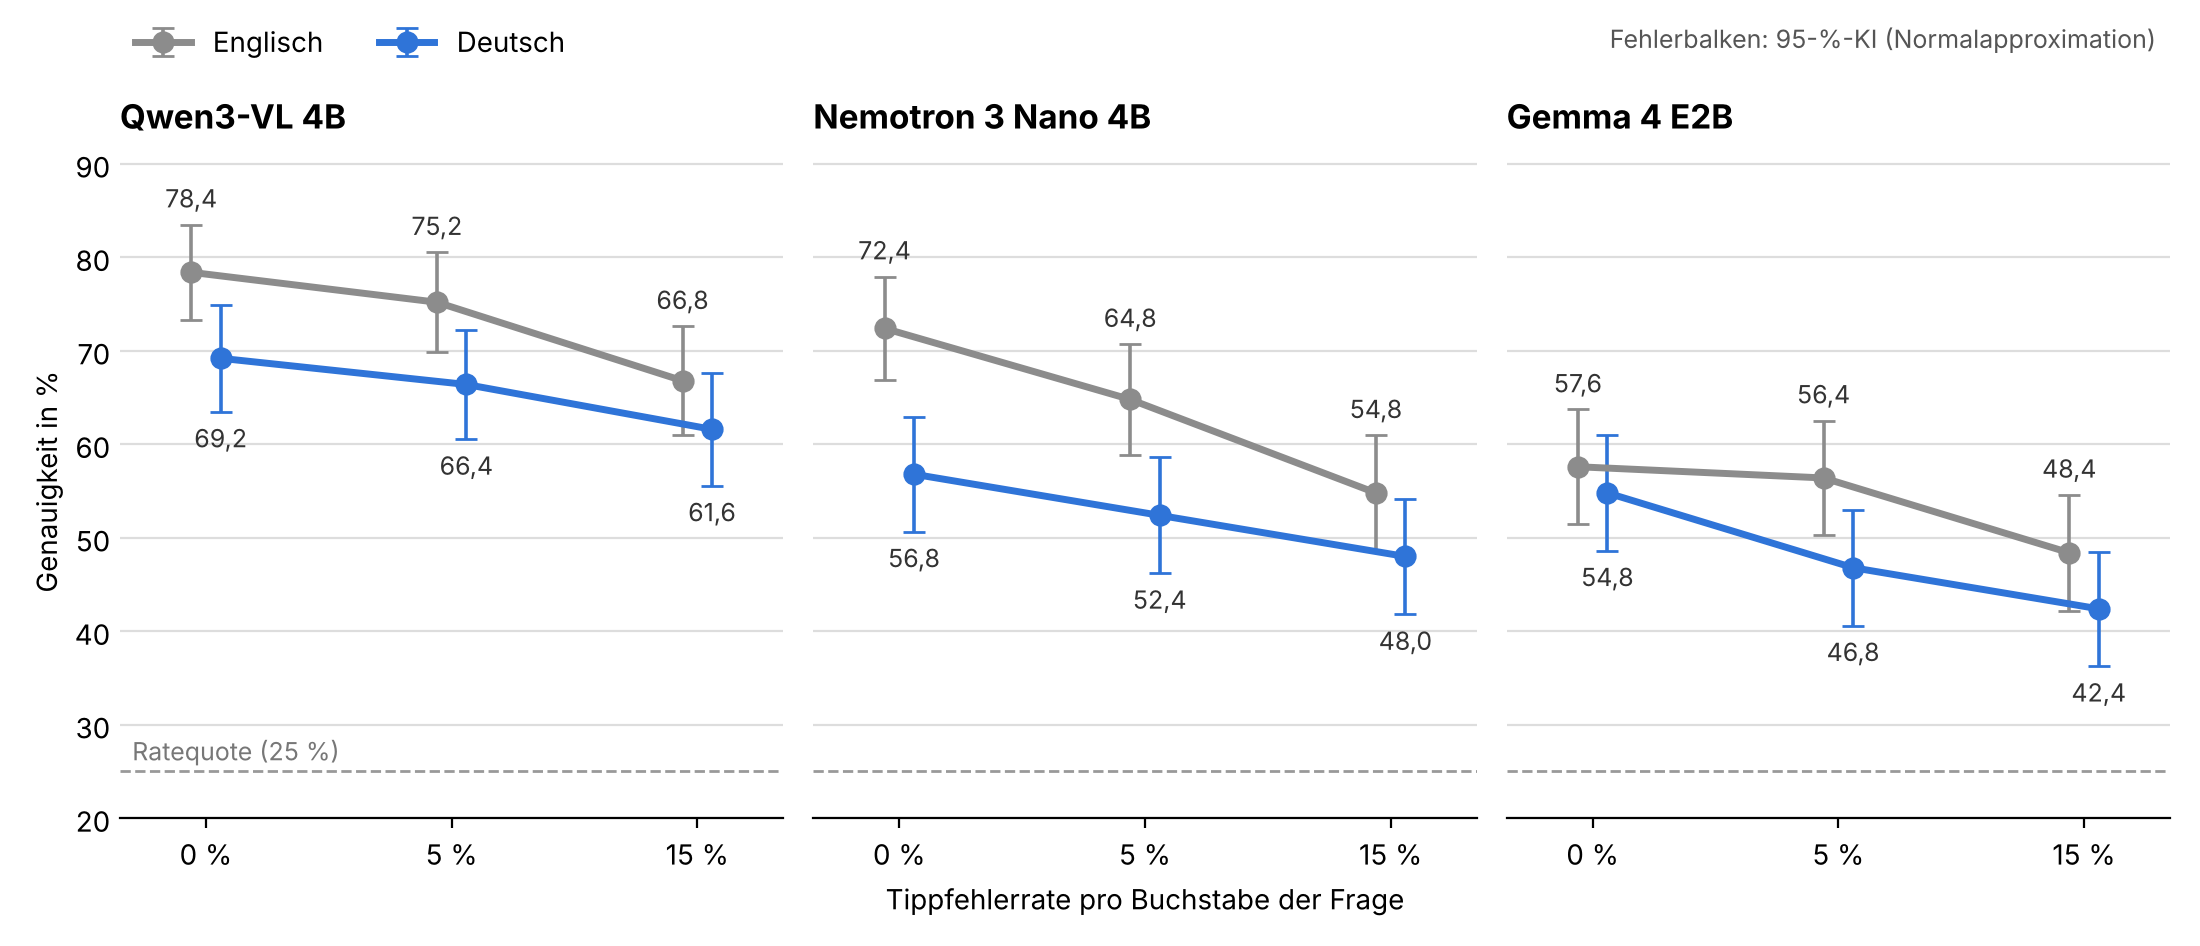
\includegraphics[width=\textwidth]{abbildung1_genauigkeit.png}
\caption{Genauigkeit nach Modell, Sprache und Tippfehlerrate (ohne Reasoning)}\label{fig:genauigkeit}
\quelle{eigene Messung, November 2026.}
\end{figure}

Tabelle~\ref{tab:kennzahlen} fasst die Kennzahlen je Modell zusammen, einschließlich des Reasoning-Durchlaufs. Die Modelle unterscheiden sich stärker in ihrer Sprachlücke als in ihrem Verlust durch Tippfehler, und welche Sprache mehr verliert, ist nicht einheitlich. Die Spalte "`Richtige pro Min."' (richtige Antworten pro Minute) bezieht sich auf den Dauerbetrieb, also ohne die erste Anfrage je Durchlauf, die die Ladezeit des Modells enthält.

\begin{table}[htbp]
\centering
\caption{Kennzahlen je Modell}\label{tab:kennzahlen}
\normalsize\setlength{\tabcolsep}{4pt}
\setstretch{1.0}\renewcommand{\arraystretch}{1.2}
\begin{tabularx}{\textwidth}{@{}lCCCCCC@{}}
\toprule
& & & \multicolumn{2}{c}{\textbf{Verlust 0 $\rightarrow$ 15~\%}} & & \\
\cmidrule(lr){4-5}
\textbf{Modell} & \textbf{Ø Genauig\-keit} & \textbf{Sprach\-lücke (pp)} & \textbf{DE / EN (pp)} & \textbf{DE / EN rel.\ (\%)} & \textbf{Laufzeit (s)} & \textbf{Richtige pro Min.} \\
\midrule
Qwen3-VL 4B             & 69,6~\% & 9,2  & 7,6 / 11,6 & 17 / 22 & 1,0  & 27,6 \\
Nemotron 3 Nano 4B      & 58,2~\% & 15,6 & 8,8 / 17,6 & 28 / 37 & 4,2  & 8,5  \\
Gemma 4 E2B             & 51,1~\% & 2,8  & 12,4 / 9,2 & 42 / 28 & 0,3  & 66,7 \\
Gemma 4 E2B (Reasoning) & 73,2~\% & 5,6 & 8,8 / 8,0  & 18 / 15 & 24,0 & 1,6  \\
\bottomrule
\end{tabularx}
\par\smallskip{\footnotesize\raggedright Anmerkungen: Ø Genauigkeit über alle sechs Bedingungen; Sprachlücke EN $-$ DE ohne Tippfehler; Verlust von 0~\% auf 15~\% Tippfehler, absolut und relativ zum Abstand von der Ratequote nach Gl.~\eqref{eq:R}; Laufzeit als Median je Frage; richtige Antworten pro Minute im Dauerbetrieb.\par}
\quelle{eigene Berechnung.}
\end{table}

\subsubsection{Spracheffekt (H1)}\label{sec:h1}

Ohne Tippfehler beantworten die Modelle deutsche Fragen im Mittel um 9,2~pp schlechter als englische (60,3~\% gegenüber 69,5~\%, $p < 0{,}001$, Tabelle~\ref{tab:haupttests}). Die Nullhypothese H1$_0$ wird damit abgelehnt, das Ergebnis spricht für H1. Je Modell ist die Lücke bei Qwen3-VL~4B und Nemotron~3 Nano~4B signifikant, bei Gemma~4 E2B nicht (Tabelle~\ref{tab:a1}). Gemma liegt allerdings auch auf Englisch nur gut 30~pp über der Ratequote.

Bei Qwen und Nemotron \textbf{schrumpft die Sprachlücke mit zunehmender Störung}, bei Nemotron von 15,6 auf 6,8~pp, bei Qwen von 9,2 auf 5,2~pp. Bei Gemma und im Mittel der drei Modelle ist sie dagegen bei 5~\% am größten (Tabelle~\ref{tab:a1}). Da dieses Muster die Wechselwirkung (H3) aus anderer Perspektive zeigt, ist es kein unabhängiger Beleg.

\subsubsection{Tippfehlereffekt (H2)}\label{sec:h2}

Bei 15~\% Tippfehlern sinkt die Genauigkeit im Mittel um 9,6~pp auf Deutsch und um 12,8~pp auf Englisch (jeweils $p < 0{,}001$, Tabelle~\ref{tab:haupttests}). Die Nullhypothese H2$_0$ wird damit für beide Sprachen abgelehnt, das Ergebnis spricht für H2. Der Rückgang ist in allen sechs Kombinationen aus Modell und Sprache signifikant, mit p-Werten zwischen $< 0{,}001$ und 0,023 (Tabelle~\ref{tab:a2}). Bei 5~\% verlieren nur Gemma auf Deutsch ($p = 0{,}008$) und Nemotron auf Englisch ($p < 0{,}001$) signifikant. In jeder Bedingung werden auch Fragen "`gewonnen"', also erst mit Tippfehlern richtig beantwortet. Manche Antworten hängen demnach eher von der Oberflächenform der Eingabe ab als von gefestigtem Wissen.

\subsubsection{Wechselwirkung von Sprache und Tippfehlern (H3)}\label{sec:h3}

Ob Deutsch stärker auf Tippfehler reagiert, lässt sich nicht einheitlich bejahen. Die Richtung des Unterschieds wechselt zwischen den Modellen (Tabelle~\ref{tab:differenz}). Alle Werte in Tabelle~\ref{tab:differenz} sind in pp angegeben. Eine negative Veränderung ist ein Rückgang, eine negative Differenz bedeutet, dass Deutsch mehr verliert. Geprüft wurde mit dem gepaarten t-Test nach Gl.~\eqref{eq:h3} und \eqref{eq:dbar} bis \eqref{eq:kit}, für "`Alle Modelle"' zusätzlich nach Gl.~\eqref{eq:mittel}.

\begin{table}[htbp]
\centering
\caption{Differenz der Rückgänge Deutsch $-$ Englisch (gepaarter t-Test)}\label{tab:differenz}
\normalsize
\setstretch{1.0}\renewcommand{\arraystretch}{1.2}
\begin{tabularx}{\textwidth}{@{}p{3.4cm}cCCCcc@{}}
\toprule
\textbf{Modell} & \textbf{Stufe} & \textbf{Verände\-rung DE} & \textbf{Verände\-rung EN} & \textbf{Differenz DE $-$ EN} & \textbf{95-\%-KI} & \textbf{p} \\
\midrule
Gemma 4 E2B        & 5~\%  & $-8{,}0$  & $-1{,}2$  & $-6{,}8$ & $[-14{,}0;\ +0{,}4]$ & 0,065 \\
Gemma 4 E2B        & 15~\% & $-12{,}4$ & $-9{,}2$  & $-3{,}2$ & $[-11{,}9;\ +5{,}5]$ & 0,47 \\
Nemotron 3 Nano 4B & 5~\%  & $-4{,}4$  & $-7{,}6$  & $+3{,}2$ & $[-3{,}0;\ +9{,}4]$  & 0,31 \\
Nemotron 3 Nano 4B & 15~\% & $-8{,}8$  & $-17{,}6$ & $+8{,}8$ & $[+1{,}1;\ +16{,}5]$ & 0,026 \\
Qwen3-VL 4B        & 5~\%  & $-2{,}8$  & $-3{,}2$  & $+0{,}4$ & $[-4{,}8;\ +5{,}6]$  & 0,88 \\
Qwen3-VL 4B        & 15~\% & $-7{,}6$  & $-11{,}6$ & $+4{,}0$ & $[-4{,}0;\ +12{,}0]$ & 0,33 \\
\midrule
\textbf{Alle Modelle} & \textbf{5~\%}  & $\boldsymbol{-5{,}1}$ & $\boldsymbol{-4{,}0}$  & $\boldsymbol{-1{,}1}$ & $\boldsymbol{[-4{,}8;\ +2{,}7]}$ & \textbf{0,58} \\
\textbf{Alle Modelle} & \textbf{15~\%} & $\boldsymbol{-9{,}6}$ & $\boldsymbol{-12{,}8}$ & $\boldsymbol{+3{,}2}$ & $\boldsymbol{[-1{,}6;\ +8{,}0]}$ & \textbf{0,19} \\
\bottomrule
\end{tabularx}
\quelle{eigene Berechnung.}
\end{table}

Nur Gemma zeigt bei 5~\% die Tendenz, dass Deutsch empfindlicher ist, knapp nicht signifikant. Bei Nemotron verliert umgekehrt Englisch bei 15~\% signifikant mehr. Über alle drei Modelle ist bei 15~\% kein Unterschied nachweisbar ($p = 0{,}19$, Tabelle~\ref{tab:haupttests}), explorativ auch bei 5~\% nicht ($p = 0{,}58$). Das Intervall bei 15~\% schließt sowohl einen kleinen Nachteil als auch einen Vorteil des Deutschen ein. Die Nullhypothese H3$_0$ wird damit \textbf{nicht abgelehnt}. Das weist nicht nach, dass beide Sprachen gleich empfindlich sind. Die Daten belegen lediglich keinen stärkeren Rückgang im Deutschen. Der beobachtete Unterschied weist in die Gegenrichtung.

Relativ zur Ratequote (Gl.~\eqref{eq:R}) verlieren beide Sprachen bei 15~\% im Mittel der drei Modelle fast denselben Anteil ihres Vorsprungs, Deutsch 27~\% und Englisch 29~\% (berechnet aus den gemittelten Genauigkeiten). Je Modell streut dieser Anteil deutlich, von 17 bzw. 22~\% bei Qwen bis 42 bzw. 28~\% bei Gemma (Tabelle~\ref{tab:kennzahlen}). In diesem Aufbau hängt die Robustheit gegenüber Tippfehlern also stärker vom Modell ab als von der Sprache. Die Sprache wirkt sich vor allem auf das Ausgangsniveau aus.

Die Ergebnisse der drei Haupttests sind Tabelle~\ref{tab:haupttests} zu entnehmen. Alle Werte sind in Prozentpunkten angegeben und über die drei Modelle nach Gl.~\eqref{eq:mittel} gemittelt. Geprüft wurde jeweils mit dem gepaarten t-Test nach Gl.~\eqref{eq:dbar} bis \eqref{eq:kit} und der Entscheidungsregel aus Abschnitt~\ref{sec:methoden}. Bei H2 bedeutet eine negative Veränderung einen Rückgang.

\begin{table}[htbp]
\centering
\caption{Haupttests zu H1 bis H3 (gepaarter t-Test, alle Modelle)}\label{tab:haupttests}
\normalsize\setlength{\tabcolsep}{4pt}
\setstretch{1.0}\renewcommand{\arraystretch}{1.2}
\begin{tabularx}{\textwidth}{@{}lLcccc>{\raggedright\arraybackslash}p{2.4cm}@{}}
\toprule
\textbf{Hypothese} & \textbf{Vergleich} & \textbf{Stufe} & $\boldsymbol{\bar{d}}$ \textbf{(pp)} & \textbf{95-\%-KI (pp)} & \textbf{p} & \textbf{Entscheidung} \\
\midrule
H1      & EN $-$ DE, Gl.~\eqref{eq:h1}          & 0~\%  & $+9{,}2$  & $[+6{,}1;\ +12{,}3]$  & $< 0{,}001$ & H1$_0$ abgelehnt \\
H2 (DE) & Veränderung DE, Gl.~\eqref{eq:h2}     & 15~\% & $-9{,}6$  & $[-13{,}4;\ -5{,}8]$  & $< 0{,}001$ & H2$_0$ abgelehnt \\
H2 (EN) & Veränderung EN, Gl.~\eqref{eq:h2}     & 15~\% & $-12{,}8$ & $[-16{,}4;\ -9{,}2]$  & $< 0{,}001$ & H2$_0$ abgelehnt \\
H3      & Differenz DE $-$ EN, Gl.~\eqref{eq:h3} & 15~\% & $+3{,}2$  & $[-1{,}6;\ +8{,}0]$   & 0,19        & H3$_0$ nicht abgelehnt \\
\bottomrule
\end{tabularx}
\quelle{eigene Berechnung.}
\end{table}

\subsubsection{Weitere Befunde}\label{sec:weitere}

\textbf{Antwortstabilität.} Bei rund der Hälfte der Fragen wechselt die Bewertung über die sechs Bedingungen mindestens einmal (Qwen 48~\%, Nemotron 50~\%, Gemma 56~\%). Mit Reasoning sinkt dieser Anteil bei Gemma auf 44~\%.

\textbf{Positionspräferenz.} Im Lösungsschlüssel ist D mit 30,0~\% die häufigste richtige Antwort, A mit 23,6~\% eine der seltensten. Nemotron wählt dagegen A am häufigsten (33,5~\%) und D am seltensten (19,7~\%). Unter seinen falschen Antworten ist A zu 40,5~\% vertreten, auf Deutsch liegt sein A-Anteil insgesamt bei rund 36~\%. Bei Qwen ist das Muster schwächer, Gemma folgt in etwa dem Schlüssel.

\textbf{Fächer.} Die Fächerwerte beruhen auf nur 50 Fragen je Fach ($\pm 14$~pp) und sind beschreibend zu lesen (Tabelle~\ref{tab:a3} im Anhang). Am meisten verlieren "`Geography"' und "`Biology"' durch Tippfehler (Ø 16,0 bzw. 14,7~pp). Den größten Spracheffekt zeigt "`Microeconomics"', bei Nemotron bis 20~pp. "`Physics"' verliert wenig (Ø 7,3~pp). Das ist aber mit Vorsicht zu lesen, weil die Werte teils nahe an der Ratequote liegen (Gemma 38 bzw. 36~\%), sodass selbst ein Rückgang auf Rateniveau dort nur wenige Prozentpunkte ausmacht. "`World History"' ist trotz der längsten Texte und meisten Tippfehler am stabilsten (Ø 3,7~pp) und liegt auf hohem Niveau. Dort schneidet Gemma auf Deutsch besser ab als auf Englisch (62 gegenüber 50~\%), was bei 50 Fragen nicht überinterpretiert werden sollte.

%%%%%%%%%%%%%%%%%%%%%%%%%%%%%%%%%%%%%%%%%%%%%%%%%%%%%%%%%

\subsection{Einfluss des Reasonings}\label{sec:reasoning}

Für diesen Vergleich wurden alle sechs Bedingungen mit Gemma~4 E2B ein zweites Mal ausgeführt, mit aktivem Nachdenkschritt und einem Limit von 2.000 Tokens. Alle übrigen Einstellungen blieben gleich. Damit ist dies der einzige Vergleich zwischen Modellkonfigurationen, in dem genau ein Merkmal variiert. Die Kennzahlen des Reasoning-Durchlaufs enthält die letzte Zeile von Tabelle~\ref{tab:kennzahlen}.

\textbf{Genauigkeit.} Mit Reasoning steigt die Genauigkeit im Mittel aller sechs Bedingungen um 22~pp. Ohne Tippfehler erreicht Gemma auf Englisch 80,0~\% statt 57,6~\% und auf Deutsch 74,4~\% statt 54,8~\%. Der Anstieg ist in jeder Bedingung signifikant ($p < 0{,}001$). Gegenüber Qwen3-VL~4B ohne Reasoning (Tabelle~\ref{tab:a1}) ist in keiner Bedingung ein signifikanter Unterschied nachweisbar ($p$ zwischen 0,16 und 0,69). Am stärksten profitieren ohne Tippfehler Fächer, in denen gerechnet oder hergeleitet wird: "`Microeconomics"' gewinnt auf Deutsch 42~pp und auf Englisch 38~pp, "`Physics"' 30~pp bzw. 26~pp. In "`Geography"' sind es nur 10~pp auf Deutsch und 12~pp auf Englisch.

\textbf{Robustheit.} Auch mit Reasoning bleibt das Modell empfindlich gegenüber Tippfehlern. Bei 15~\% sinkt die Genauigkeit in beiden Sprachen signifikant (jeweils $p = 0{,}005$), auf Deutsch um 8,8~pp auf 65,6~\% und auf Englisch um 8,0~pp auf 72,0~\%. Der absolute Verlust fällt damit etwas geringer aus als ohne Reasoning (12,4 bzw. 9,2~pp). Relativ zum Abstand von der Ratequote ist er dagegen deutlich kleiner (Tabelle~\ref{tab:kennzahlen}): Auf Deutsch verliert das Modell 18~\% statt 42~\% seines Vorsprungs, auf Englisch 15~\% statt 28~\%. Ob sich die Rückgänge mit und ohne Reasoning signifikant unterscheiden, wurde nicht gesondert getestet. Das Sprachmuster bleibt erhalten. Ohne Tippfehler ist Deutsch weiterhin signifikant schlechter ($-5{,}6$~pp, $p = 0{,}03$). Die Wechselwirkung ist erneut nicht signifikant ($p = 0{,}22$ bei 5~\%, $p = 0{,}84$ bei 15~\%).

\textbf{Leere Antworten und Rechenaufwand.} Alle 12 leeren Antworten betreffen "`Physics"' und dauerten 84 bis 107 Sekunden. Das Modell verbrauchte hier offenbar das Token-Limit vollständig zum Nachdenken. Selbst wenn alle diese Antworten richtig gewesen wären, läge die Genauigkeit je Bedingung um höchstens 1,6~pp höher. Im Median benötigte Gemma mit Reasoning 24 Sekunden pro Frage statt 0,3 Sekunden, also rund 80-mal so lange. Auf Deutsch dauerte eine Antwort länger als auf Englisch (26,0 gegenüber 21,4 Sekunden ohne Tippfehler).

\newpage
%%%%%%%%%%%%%%%%%%%%%%%%%%%%%%%%%%%%%%%%%%%%%%%%%%%%%%%%%
%%%%%%%%%%%%%%%%%%%%%%%%%%%%%%%%%%%%%%%%%%%%%%%%%%%%%%%%%

\section{Diskussion}\label{sec:diskussion}

%%%%%%%%%%%%%%%%%%%%%%%%%%%%%%%%%%%%%%%%%%%%%%%%%%%%%%%%%

\subsection{Einordnung des Spracheffekts}\label{sec:einordnung-sprache}

Der Spracheffekt ist das deutlichste Ergebnis und entspricht der in Abschnitt~\ref{sec:hypothesen} hergeleiteten Erwartung. Ob die für Llama~2 dokumentierte Dominanz englischer Trainingsdaten \citep{touvron_llama_2023} in ähnlichem Umfang für die hier untersuchten Modelle gilt, lässt sich daraus allerdings nicht ableiten. Daneben kann die Tokenisierung eine Rolle spielen, da derselbe Inhalt je nach Sprache in unterschiedlich lange Tokenfolgen zerlegt wird \citep{petrov_language_2023}. Seltene oder zusammengesetzte Fachwörter wie "`Kreuzpreiselastizität"' werden dabei in mehrere Teilwörter zerlegt \citep{sennrich_neural_2016}. Ob diese Segmentierung zum Leistungsunterschied beiträgt, wurde hier nicht gesondert untersucht. Damit vereinbar ist, dass der Spracheffekt in "`Microeconomics"' am größten ist, wo Fachbegriffe die Lösung tragen.

Die besonders große Lücke bei Nemotron (15,6~pp) könnte auf Unterschiede in der Mehrsprachigkeit des Trainings zurückgehen. Dazu passt, dass die Model Card als unterstützte Sprache nur Englisch nennt und das Modell für Englisch und Programmiersprachen vorsieht, obwohl die Nachtrainingsdaten auch deutsche Texte umfassen \citep{noauthor_nvidianvidia-nemotron-3-nano-4b-bf16_2026}. In der Positionsanalyse wählt Nemotron unter seinen falschen Antworten überdurchschnittlich oft Option A, auf Deutsch insgesamt in rund 36~\% der Fälle. Das ist damit vereinbar, dass das Modell bei Unsicherheit auf A ausweicht und auf Deutsch häufiger unsicher ist. Solche Präferenzen für bestimmte Antwortbuchstaben sind bei Multiple-Choice-Aufgaben gut dokumentiert \citep{zheng_large_2024, pezeshkpour_large_2023}. Die Positionspräferenz dürfte die Sprachlücke daher nicht verursachen. Sie beeinflusst vielmehr, in welche falschen Antworten die Unsicherheit mündet, und kann die Lücke leicht vergrößern, da A im Lösungsschlüssel unterdurchschnittlich oft richtig ist. Die kleine Sprachlücke bei Gemma fällt mit einem niedrigen englischen Ausgangsniveau von nur gut 30~pp über der Ratequote zusammen. Damit vereinbar ist, dass die Lücke mit Reasoning und höherem Ausgangsniveau von 2,8 auf 5,6~pp wächst (Tabelle~\ref{tab:kennzahlen}). Ob dafür das niedrigere Niveau oder andere modellspezifische Eigenschaften verantwortlich sind, lässt sich mit diesem Aufbau jedoch nicht entscheiden.

%%%%%%%%%%%%%%%%%%%%%%%%%%%%%%%%%%%%%%%%%%%%%%%%%%%%%%%%%

\subsection{Einordnung von Tippfehlereffekt und Wechselwirkung}\label{sec:einordnung-tippfehler}

Eine Tippfehlerrate von 15~\% schwächt alle Modelle, ein großer Teil der Leistung bleibt jedoch erhalten. Obwohl rechnerisch etwa jedes zweite längere Wort gestört ist (Kasten~1), erreicht Qwen noch 62 bis 67~\%. Offenbar können die Modelle viele gestörte Wörter aus dem Kontext erschließen, solange die tragenden Begriffe erkennbar bleiben. "`World History"' ist trotz der meisten Tippfehler am stabilsten. Eine mögliche Erklärung ist die Redundanz langer Quelltexte. Kurze Fragen, deren Lösung an einem Fachbegriff hängt, sind dagegen anfällig, wenn genau dieser Begriff gestört wird. Außerdem bleiben die Antwortoptionen fehlerfrei. Wo sie schon für sich viel über die Lösung verraten, schaden Tippfehler im Fragetext wenig.

Die Nullhypothese H3$_0$ konnte nicht abgelehnt werden. Mit nur einem Modell (Gemma) hätte man eher eine höhere Empfindlichkeit des Deutschen vermutet. Erst Qwen und Nemotron deuten darauf hin, dass dieser Befund modellspezifisch ist. Dass Englisch in Prozentpunkten teilweise mehr verliert, ist mit dem höheren Ausgangsniveau vereinbar: Relativ zum Abstand von der Ratequote verlieren beide Sprachen einen ähnlichen Anteil ihres Genauigkeitsvorsprungs (Abschnitt~\ref{sec:h3}). Zusätzlich könnte die englische Leistung teilweise auf der Wiedererkennung bekannter Originalfragen beruhen, die Tippfehler stören \citep{deng_investigating_2024}. Dabei enthielten die deutschen Fragen wegen der buchstabenbezogenen Fehlerrate mehr Tippfehler (bei 15~\% im Median 18,5 gegenüber 15). Pro einzelnem Fehler spricht das eher für eine geringere als für eine höhere Empfindlichkeit des Deutschen. Ein Vergleich bei gleicher Fehlerzahl je Frage war allerdings nicht Teil des Versuchsplans. Der Abstand zwischen den Sprachen zeigt sich in diesem Aufbau also vor allem bereits bei der fehlerfreien Frage. Das deckt sich mit \citet{zhao_evaluating_2026}, bei denen die gut vertretenen Sprachen Englisch, Deutsch und Französisch vergleichsweise geringe Einbußen zeigen und Deutsch nicht einheitlich mehr verliert als Englisch. Auch \citet{aliakbarzadeh_exploring_2025} finden Englisch gegenüber realen Schreibfehlern weniger robust als andere Sprachen, darunter Deutsch, allerdings an anderen Modellen und Aufgaben. Der Vorteil ressourcenstarker Sprachen betrifft vor allem den Vergleich mit Sprachen wie Arabisch oder Hindi. Für die Praxis ist außerdem die Instabilität einzelner Antworten relevant. Auch bei einer mittleren Genauigkeit von 70~\% kann eine konkrete Antwort bei leicht veränderter Eingabe kippen. Auf eine solche Instabilität setzen Angriffe, die viele zufällig veränderte Varianten einer Eingabe durchprobieren \citep{hughes_best--n_2024}.

%%%%%%%%%%%%%%%%%%%%%%%%%%%%%%%%%%%%%%%%%%%%%%%%%%%%%%%%%

\subsection{Nutzen und Aufwand des Reasonings}\label{sec:nutzen-reasoning}

Zwischen Gemma mit Reasoning und Qwen ohne Reasoning ließ sich trotz der geringeren effektiven Parameterzahl von Gemma in keiner Bedingung ein signifikanter Unterschied nachweisen. Die beobachteten Genauigkeiten liegen auf vergleichbarem Niveau, eine Gleichwertigkeit ist damit jedoch nicht belegt. Beschreibend glich der Antwortmodus den Rückstand von Gemma gegenüber dem größeren Modell aus, was mit den Befunden zum Einsatz von Rechenaufwand zur Laufzeit vereinbar ist \citep{snell_scaling_2024}. Eine allgemeine Aussage, dass Reasoning wichtiger sei als Modellgröße, lässt sich aus einem einzelnen Modell jedoch nicht ableiten. Die Ergebnisse sprechen eher dafür, dass ein Reasoning-Modell, das zur direkten Antwort gezwungen wird, deutlich unter seinen Möglichkeiten arbeitet. Der große Gewinn in "`Microeconomics"' und "`Physics"' passt zu dem Befund, dass vor allem Aufgaben mit Rechen- oder Herleitungsanteil von Zwischenschritten profitieren \citep{sprague_cot_2025}. In "`Geography"', wo vor allem Faktenwissen gefragt ist, fällt der Gewinn mit 10 bzw. 12~pp geringer aus.

Aus betriebswirtschaftlicher Sicht ergibt sich ein \textbf{Zielkonflikt zwischen Genauigkeit und Durchsatz} (Tabelle~\ref{tab:kennzahlen}). Gemma liefert ohne Reasoning rund 67 richtige Antworten pro Minute, mit Reasoning 1,6, also etwa ein Vierzigstel, bei rund 22~pp höherer Genauigkeit. Gegenüber Qwen bringt Reasoning im Mittel nur 3,6~pp mehr (73,2 gegenüber 69,6~\%) bei etwa 24-facher Median-Laufzeit. Nemotron ist Qwen in diesem Aufbau in beiden Dimensionen unterlegen, wobei der Laufzeitvergleich eingeschränkt ist, weil Nemotron als GGUF-Datei über eine andere Laufzeitumgebung lief als die MLX-Modelle.

Was diese Ergebnisse für die Praxis bedeuten könnten, lässt sich an einem hypothetischen Szenario zeigen. Ein Unternehmen will einen deutschsprachigen Assistenten für Kundenanfragen lokal auf Standard-Hardware betreiben. Die folgenden Überlegungen übertragen die Befunde dieser Arbeit auf diesen Fall. Geprüft wurden sie an echten Kundenanfragen nicht, und MMLU-Wissensfragen unterscheiden sich von solchen Anfragen in Inhalt und Format.

Erstens dürften Ergebnisse englischsprachiger Benchmarks die Leistung bei deutscher Nutzung überschätzen. In diesem Aufbau lag die Genauigkeit auf Deutsch im Mittel 9,2~pp niedriger (Abschnitt~\ref{sec:h1}). Zweitens enthalten reale Eingaben regelmäßig Tippfehler, wenn auch meist deutlich weniger als in den hier gewählten Belastungsstufen (Abschnitt~\ref{sec:hypothesen}). Da in den Versuchen bei rund der Hälfte der Fragen die Bewertung mindestens einmal wechselte (Abschnitt~\ref{sec:weitere}), sollten Antworten mit hohen Fehlerkosten, etwa zu Preisen oder Vertragsbedingungen, nicht ungeprüft ausgegeben werden. Drittens hängt die Modellwahl vom Verhältnis zwischen Anfragevolumen und Fehlerkosten ab. Qwen liefert in diesem Aufbau 27,6 richtige Antworten pro Minute, Gemma mit Reasoning 1,6 bei 3,6~pp höherer mittlerer Genauigkeit (Tabelle~\ref{tab:kennzahlen}). Bei vielen einfachen Anfragen spräche das für ein schnelles, direkt antwortendes Modell wie Qwen. Bei wenigen Anfragen mit teuren Fehlentscheidungen könnte sich der vielfache Rechenaufwand des Reasonings lohnen.

%%%%%%%%%%%%%%%%%%%%%%%%%%%%%%%%%%%%%%%%%%%%%%%%%%%%%%%%%

\subsection{Grenzen der Untersuchung}\label{sec:grenzen}

\begin{itemize}
\item \textbf{Stichprobe und Testanzahl:} 250 Fragen reichen für die Haupteffekte, aber nicht, um eine Wechselwirkung von wenigen pp sicher nachzuweisen. Pro Fach sind es nur 50 Fragen. Neben den drei Haupttests wurden zahlreiche explorative Tests ohne Korrektur für multiples Testen durchgeführt. Ergebnisse knapp unter $p = 0{,}05$ (z.\,B. bei Nemotron bei 15~\%) sind daher als Hinweise zu lesen. Zudem gab es pro Bedingung nur einen deterministischen Durchlauf.

\item \textbf{Modelle:} Größe, Architektur, Trainingsdaten, Reasoning-Auslegung und Laufzeitformat variieren gleichzeitig, sodass sich Modellunterschiede keinem einzelnen Merkmal zuordnen lassen. Nur der Reasoning-Vergleich bei Gemma hält alles andere konstant. Nemotron wurde nur ohne Reasoning getestet. Seine Laufzeit schwankt für dieselbe Frage stark (bei Frage 688 zwischen 1,4 und 16,2 Sekunden). Ob es trotz Deaktivierung intern zusätzliche Tokens erzeugt hat, wurde nicht geprüft. Der Reasoning-Durchlauf von Gemma lief wie alle übrigen mit Temperatur 0, obwohl die Model Card eine Temperatur von 1,0 empfiehlt \citep{deepmind_gemma_nodate}. Ob dies die Genauigkeit oder die Länge der Denkketten beeinflusst hat, etwa bei den zwölf leeren Antworten, wurde nicht geprüft.

\item \textbf{Übersetzung:} Die deutsche Fassung ist eine korrigierte maschinelle Übersetzung US-geprägter Inhalte. Trotz manueller Prüfung können Übersetzungsartefakte verbleiben \citep{artetxe_translation_2020}, sodass ein Teil der gemessenen Sprachlücke auf die Übersetzung statt auf die Sprache zurückgehen könnte.

\item \textbf{Fehlermodell:} Simuliert wurde nur ein Fehlertyp (Nachbartaste), gleichmäßig verteilt. Echte Tippfehler umfassen auch Auslassungen und Vertauschungen. Die Fehlerstufen sind Belastungsstufen und liegen deutlich über beobachteten Fehlerraten realer Eingaben. Da die Fehler zufällig und nicht gezielt gesetzt wurden, bilden die Ergebnisse nur eine Untergrenze adversarialer Risiken innerhalb desselben Störungsraums; über andere Angriffsziele wie Jailbreaks erlauben sie keine Aussage (Abschnitt~\ref{sec:robustheit}). Wegen der buchstabenbezogenen Rate erhielten deutsche Fragen zudem mehr Fehler als englische.

\item \textbf{Antwortformat und Messung:} Die Antwort mit einem Buchstaben misst das Wiedererkennen der richtigen Option. Positionspräferenzen und der ungleich verteilte Lösungsschlüssel können die Werte verzerren. Andere Formulierungen der Anweisung wurden nicht geprüft.
\end{itemize}

\newpage
%%%%%%%%%%%%%%%%%%%%%%%%%%%%%%%%%%%%%%%%%%%%%%%%%%%%%%%%%
%%%%%%%%%%%%%%%%%%%%%%%%%%%%%%%%%%%%%%%%%%%%%%%%%%%%%%%%%

\section{Fazit und Ausblick}\label{sec:fazit}

Untersucht wurde, wie robust kleine, lokal betriebene Sprachmodelle gegenüber einem Sprachwechsel und gegenüber Tippfehlern sind.

Kleine Sprachmodelle sind auf Deutsch messbar schwächer als auf Englisch (H1$_0$ abgelehnt), und Tippfehler schwächen sie in beiden Sprachen (H2$_0$ abgelehnt). Eine generell höhere Empfindlichkeit des Deutschen gegenüber Tippfehlern zeigt sich nicht (H3$_0$ nicht abgelehnt): Relativ zum Abstand von der Ratequote verlieren beide Sprachen einen ähnlichen Anteil ihres Genauigkeitsvorsprungs, und bei zwei von drei Modellen schrumpft die Sprachlücke mit zunehmender Störung. Der Nachteil deutscher Eingaben zeigt sich in diesem Aufbau also vor allem im niedrigeren Ausgangsniveau, und wie robust ein System gegenüber Tippfehlern ist, hängt stärker vom Modell ab als von der Sprache.

Den größten Einfluss auf die Genauigkeit hatte das Reasoning. Es hob ein kleines Modell um rund 22~pp und vervielfachte die Rechenzeit. Tippfehler senkten die Genauigkeit auch mit Reasoning signifikant; der absolute Verlust fiel etwas, der Verlust relativ zur Ratequote deutlich geringer aus. Methodisch zeigt sich, dass Befunde an einem einzelnen Modell nur eingeschränkt verallgemeinerbar sind: Der bei Gemma beobachtete stärkere Verlust auf Deutsch wiederholte sich bei zwei weiteren Modellen nicht.

Anschlussarbeiten sollten den Reasoning-Vergleich auf weitere Modelle ausweiten, größere Modelle, weitere Fehlertypen und permutierte Antwortreihenfolgen einbeziehen sowie original deutschsprachige Benchmarks statt Übersetzungen verwenden. Da die Tippfehler hier zufällig gesetzt wurden, wäre zudem zu prüfen, wie stark gezielt platzierte Störungen mit demselben Budget die Modelle treffen. Ebenso wäre direkt zu testen, ob Reasoning den Verlust durch Tippfehler verringert.

Über Texteingaben hinaus lässt sich der Versuchsaufbau auf andere Modalitäten übertragen. In der Bildverarbeitung entsprechen den Tippfehlern natürliche Bildstörungen wie Rauschen, Unschärfe, Kompressionsartefakte oder veränderte Helligkeit, die im Betrieb ohne Täuschungsabsicht entstehen. Hendrycks und Dietterich \citeyearpar{hendrycks_benchmarking_2019} haben solche Störungen in 15 Störungsarten mit jeweils fünf Schweregraden standardisiert. Diese Schweregrade wären das Gegenstück zu den hier verwendeten Fehlerstufen. Das Gegenstück zum Sprachwechsel wäre eine Verschiebung der Bilddomäne, etwa von Fotos zu Skizzen. Dabei bleibt der Inhalt gleich, während sich seine Darstellung vom Schwerpunkt der Trainingsdaten entfernt. Da adversariale Störungen vor allem in der Bildverarbeitung erforscht wurden \citep{goodfellow_explaining_2014}, ließe sich auch die hier gewählte Logik einer Untergrenze für adversariale Risiken innerhalb desselben Störungsraums übertragen. Naheliegend wäre ein Versuch mit Bild-Sprach-Modellen wie dem hier eingesetzten Qwen3-VL \citep{bai_qwen3-vl_2025}, bei dem dieselben Fragen als Bild gestellt, etwa als Foto eines Aufgabenblatts, und mit Bildstörungen versehen werden. So ließe sich prüfen, ob die Robustheit auch bei Störungen der Darstellung statt des Textes stärker vom Modell als von der Eingabesprache abhängt.

\newpage

%%%%%%%%%%%%%%%%%%%%%%%%%%%%%%%%%%%%%%%%%%%%%%%%%%%%%%%%%
%%%%%%%%%%%%%%%%%%%%%%%%%%%%%%%%%%%%%%%%%%%%%%%%%%%%%%%%%

\section*{Anhang A}
\addcontentsline{toc}{section}{Anhang A}

\setcounter{table}{0}
\renewcommand{\thetable}{A\arabic{table}}

Tabelle~\ref{tab:a1} zeigt die Sprachlücke je Modell und Fehlerstufe, geprüft mit dem exakten McNemar-Test nach Gl.~\eqref{eq:mcnemar}. Bei Nemotron mit 15~\% Tippfehlern liegt der p-Wert ungerundet bei 0,0498.

\begin{table}[htbp]
\centering
\caption{Sprachlücke Englisch $-$ Deutsch je Fehlerstufe (exakter McNemar-Test)}\label{tab:a1}
\normalsize
\setstretch{1.0}\renewcommand{\arraystretch}{1.2}
\begin{tabularx}{\textwidth}{@{}p{3.4cm}cccCCCc@{}}
\toprule
\textbf{Modell} & \textbf{Stufe} & \textbf{EN} & \textbf{DE} & \textbf{$\Delta$ EN $-$ DE (pp)} & \textbf{nur EN richtig} & \textbf{nur DE richtig} & \textbf{p} \\
\midrule
Qwen3-VL 4B        & 0~\%  & 78,4~\% & 69,2~\% & 9,2  & 32 & 9  & $< 0{,}001$ \\
                   & 5~\%  & 75,2~\% & 66,4~\% & 8,8  & 40 & 18 & 0,005 \\
                   & 15~\% & 66,8~\% & 61,6~\% & 5,2  & 47 & 34 & 0,18 \\
\addlinespace
Nemotron 3 Nano 4B & 0~\%  & 72,4~\% & 56,8~\% & 15,6 & 47 & 8  & $< 0{,}001$ \\
                   & 5~\%  & 64,8~\% & 52,4~\% & 12,4 & 47 & 16 & $< 0{,}001$ \\
                   & 15~\% & 54,8~\% & 48,0~\% & 6,8  & 42 & 25 & $< 0{,}05$ \\
\addlinespace
Gemma 4 E2B        & 0~\%  & 57,6~\% & 54,8~\% & 2,8  & 32 & 25 & 0,43 \\
                   & 5~\%  & 56,4~\% & 46,8~\% & 9,6  & 46 & 22 & 0,005 \\
                   & 15~\% & 48,4~\% & 42,4~\% & 6,0  & 46 & 31 & 0,11 \\
\midrule
\textbf{Mittel (3 Modelle)} & \textbf{0~\%}  & & & \textbf{9,2}  & & & \\
                            & \textbf{5~\%}  & & & \textbf{10,3} & & & \\
                            & \textbf{15~\%} & & & \textbf{6,0}  & & & \\
\bottomrule
\end{tabularx}
\quelle{eigene Berechnung.}
\end{table}

Tabelle~\ref{tab:a2} zeigt den Rückgang durch Tippfehler je Modell und Sprache, ebenfalls geprüft mit dem exakten McNemar-Test nach Gl.~\eqref{eq:mcnemar}. "`Verloren"' bezeichnet Fragen, die ohne Tippfehler richtig und mit Tippfehlern falsch beantwortet wurden, "`gewonnen"' den umgekehrten Fall.

\begin{table}[htbp]
\centering
\caption{Rückgang durch Tippfehler je Modell und Sprache (exakter McNemar-Test)}\label{tab:a2}
\normalsize
\setstretch{1.0}\renewcommand{\arraystretch}{1.2}
\begin{tabularx}{\textwidth}{@{}p{3.2cm}cCcCc@{}}
\toprule
\textbf{Modell} & \textbf{Sprache} & \textbf{0 $\rightarrow$ 5~\%: verloren / gewonnen} & \textbf{p} & \textbf{0 $\rightarrow$ 15~\%: verloren / gewonnen} & \textbf{p} \\
\midrule
Qwen3-VL 4B        & EN & 13 / 5  & 0,10        & 38 / 9  & $< 0{,}001$ \\
Qwen3-VL 4B        & DE & 21 / 14 & 0,31        & 41 / 22 & 0,023 \\
Nemotron 3 Nano 4B & EN & 25 / 6  & $< 0{,}001$ & 55 / 11 & $< 0{,}001$ \\
Nemotron 3 Nano 4B & DE & 24 / 13 & 0,10        & 40 / 18 & 0,005 \\
Gemma 4 E2B        & EN & 18 / 15 & 0,73        & 40 / 17 & 0,003 \\
Gemma 4 E2B        & DE & 36 / 16 & 0,008       & 54 / 23 & $< 0{,}001$ \\
\bottomrule
\end{tabularx}
\quelle{eigene Berechnung.}
\end{table}

Tabelle~\ref{tab:a3} zeigt die Genauigkeit je Fach. Die Spalte "`Ø Veränderung"' gibt das Mittel über die drei abgebildeten Modelle und beide Sprachen an, ohne Gemma mit Reasoning.

\begin{table}[htbp]
\centering
\caption{Genauigkeit nach Fach in \%, ohne Tippfehler und bei 15~\% (jeweils EN / DE)}\label{tab:a3}
\normalsize\setlength{\tabcolsep}{4pt}
\setstretch{1.0}\renewcommand{\arraystretch}{1.2}
\begin{tabularx}{\textwidth}{@{}p{2.5cm}CCCCCCC@{}}
\toprule
\textbf{Fach} & \textbf{Qwen 0~\%} & \textbf{Qwen 15~\%} & \textbf{Nemo\-tron 0~\%} & \textbf{Nemo\-tron 15~\%} & \textbf{Gemma 0~\%} & \textbf{Gemma 15~\%} & \textbf{Ø Verände\-rung 0 $\rightarrow$ 15~\% (pp)} \\
\midrule
Biology        & 88 / 82 & 82 / 74 & 80 / 62 & 56 / 42 & 72 / 68 & 60 / 50 & $-14{,}7$ \\
Geography      & 86 / 78 & 72 / 62 & 84 / 72 & 68 / 66 & 76 / 70 & 60 / 42 & $-16{,}0$ \\
Microeconomics & 78 / 68 & 54 / 50 & 66 / 46 & 46 / 32 & 52 / 38 & 40 / 40 & $-14{,}3$ \\
Physics        & 60 / 48 & 50 / 50 & 56 / 44 & 32 / 44 & 38 / 36 & 32 / 30 & $-7{,}3$ \\
World History  & 80 / 70 & 76 / 72 & 76 / 60 & 72 / 56 & 50 / 62 & 50 / 50 & $-3{,}7$ \\
\bottomrule
\end{tabularx}
\quelle{eigene Berechnung.}
\end{table}

\clearpage

%%%%%%%%%%%%%%%%%%%%%%%%%%%%%%%%%%%%%%%%%%%%%%%%%%%%%%%%%
%%%%%%%%%%%%%%%%%%%%%%%%%%%%%%%%%%%%%%%%%%%%%%%%%%%%%%%%%

\section*{Anhang B}
\addcontentsline{toc}{section}{Anhang B}

\textbf{Angaben zur Reproduzierbarkeit.} Die folgenden Angaben ergänzen Abschnitt~\ref{sec:versuchsaufbau} und \ref{sec:methoden}.

\begin{itemize}
\item \textbf{Datensatz:} \texttt{cais/mmlu} auf Hugging Face \citep{hendrycks_measuring_2021}, Test-Split, Commit \texttt{\small c30699e8356da336a370243923dbaf21066bb9fe}; Ziehung von 50 Fragen je Fach mit Seed 42.
\item \textbf{Modelle:} über den integrierten Modellkatalog von LM Studio heruntergeladen; Modellkennungen, Formate und Quantisierung siehe Tabelle~\ref{tab:modelle}. Da LM Studio keine Revisionsangaben ausweist, sind die Modelldateien durch Kennung und Quantisierung bestimmt.
\item \textbf{Laufzeitumgebung:} LM Studio 0.4.26 (Build 4) auf einem MacBook Air M1 mit 8~GB Arbeitsspeicher, macOS 26.6.2.
\item \textbf{Abfrage:} Temperatur 0, Seed 42, jede Frage als einzelne Anfrage über die API von LM Studio. Token-Limit ohne Reasoning 2, mit Reasoning 2.000. Der Reasoning-Modus wurde über die Modelleinstellungen in LM Studio ein- bzw. ausgeschaltet.
\item \textbf{Auswertung:} Microsoft Excel für Mac, Version 16.115.2 (26112215); alle Kennzahlen und Tests als Formeln in der Auswertungsdatei (Excel-Arbeitsmappe).
\item \textbf{Software für die Datenaufbereitung und Abfrage:} Python 3.9.6 mit pandas 2.3.3, openpyxl 3.1.5, openai 2.48.0 (Zugriff auf die API von LM Studio) und deepl 1.33.0 (Zugriff auf die DeepL-API).
\end{itemize}

\textbf{Skripte.} Die Versuchsdurchführung beruht auf fünf Python-Skripten, die der Arbeit in elektronischer Form beiliegen:

\begin{itemize}
\item \texttt{stichprobe\_ziehen.py}: Ziehung von 50 Fragen je Fach mit Seed 42 und Aufteilung der Antwortoptionen in die Spalten A--D.
\item \texttt{uebersetzen.py}: feldweise Übersetzung von Fragen und Antwortoptionen ins Deutsche mit der DeepL-API (durchgeführt am 22.11.2026); die anschließende manuelle Korrektur erfolgte direkt in der Excel-Datei.
\item \texttt{tippfehler\_einbauen.py}: Erzeugung der Fehlerstufen 5~\% und 15~\% durch Nachbartastenfehler (QWERTZ bzw. QWERTY) mit festem Seed je Frage.
\item \texttt{pruefen.py}: Kontrolle der erzeugten Tippfehler (nur zulässige Stellen und Nachbartasten, korrekte Fehlerzahl, 5-\%-Stufe als Teilmenge der 15-\%-Stufe, identische Fragen über alle Modelle).
\item \texttt{mmlu\_an\_llm.py}: Abfrage der Modelle über die API von LM Studio, Auslesen des Antwortbuchstabens und Bewertung.
\end{itemize}

\textbf{Wortlaut der Anweisungen.} Systemanweisung und Prompt wurden in der Sprache der Frage gestellt. Die Platzhalter in geschweiften Klammern wurden durch den Fragetext und die vier Antwortoptionen ersetzt.

\begin{center}
\normalsize\setstretch{1.0}\renewcommand{\arraystretch}{1.2}
\begin{tabularx}{\textwidth}{@{}>{\raggedright\arraybackslash}X>{\raggedright\arraybackslash}X@{}}
\toprule
\textbf{Deutsch} & \textbf{Englisch} \\
\midrule
\textbf{System:} Du bist ein hilfreicher Assistent. Du beantwortest Multiple-Choice-Fragen.
& \textbf{System:} You are a helpful assistant. You answer multiple-choice questions. \\
\addlinespace
\textbf{Prompt:} Beantworte die folgende Multiple-Choice-Frage. Antworte ausschließlich mit dem Buchstaben der richtigen Antwort (A, B, C oder D), ohne Erklärung.\newline\newline
Frage: \{question\}\newline\newline
A) \{A\}\newline B) \{B\}\newline C) \{C\}\newline D) \{D\}\newline\newline
Antwort:
& \textbf{Prompt:} Answer the following multiple-choice question. Respond only with the letter of the correct answer (A, B, C, or D), without explanation.\newline\newline
Question: \{question\}\newline\newline
A) \{A\}\newline B) \{B\}\newline C) \{C\}\newline D) \{D\}\newline\newline
Answer: \\
\bottomrule
\end{tabularx}
\end{center}

\newpage

%%%%%%%%%%%%%%%%%%%%%%%%%%%%%%%%%%%%%%%%%%%%%%%%%%%%%%%%%
%%%%%%%%%%%%%%%%%%%%%%%%%%%%%%%%%%%%%%%%%%%%%%%%%%%%%%%%%

\addcontentsline{toc}{section}{Literaturverzeichnis}
\bibliographystyle{plainnat}   % or another NatBib‐compatible style
\bibliography{literature}       % ohne .bib-Endung

\newpage

%%%%%%%%%%%%%%%%%%%%%%%%%%%%%%%%%%%%%%%%%%%%%%%%%%%%%%%%%
%%%%%%%%%%%%%%%%%%%%%%%%%%%%%%%%%%%%%%%%%%%%%%%%%%%%%%%%%

\section*{Eidesstattliche Erklärung}
\addcontentsline{toc}{section}{Eidesstattliche Erklärung}

\glqq Ich versichere, dass ich die vorstehende Arbeit selbstständig und
ohne fremde Hilfe angefertigt und mich anderer als der im beigefügten
Verzeichnis angegebenen Hilfsmittel nicht bedient habe. Alle Stellen, die
wörtlich oder sinngemäß aus Veröffentlichungen übernommen wurden, sind als
solche kenntlich gemacht. Alle Internetquellen sind der Arbeit beigefügt.
Des Weiteren versichere ich, dass ich die Arbeit vorher nicht in einem anderen
Prüfungsverfahren eingereicht habe und dass die eingereichte schriftliche Fassung
der auf dem elektronischen Speichermedium entspricht.\grqq
~\\[15mm]
\begin{tabbing}
\hspace*{6cm}\=\kill
Hamburg, 27.11.2026 \> \rule{6cm}{0.4pt}\\
                    \> Kirill Titov\\[15mm]
Hamburg, 27.11.2026 \> \rule{6cm}{0.4pt}\\
                    \> Talip Dablan
\end{tabbing}


\end{document}
